\documentclass[1p]{elsarticle_modified}
%\bibliographystyle{elsarticle-num}

%\usepackage[colorlinks]{hyperref}
%\usepackage{abbrmath_seonhwa} %\Abb, \Ascr, \Acal ,\Abf, \Afrak
\usepackage{amsfonts}
\usepackage{amssymb}
\usepackage{amsmath}
\usepackage{amsthm}
\usepackage{scalefnt}
\usepackage{amsbsy}
\usepackage{kotex}
\usepackage{caption}
\usepackage{subfig}
\usepackage{color}
\usepackage{graphicx}
\usepackage{xcolor} %% white, black, red, green, blue, cyan, magenta, yellow
\usepackage{float}
\usepackage{setspace}
\usepackage{hyperref}

\usepackage{tikz}
\usetikzlibrary{arrows}

\usepackage{multirow}
\usepackage{array} % fixed length table
\usepackage{hhline}

%%%%%%%%%%%%%%%%%%%%%
\makeatletter
\renewcommand*\env@matrix[1][\arraystretch]{%
	\edef\arraystretch{#1}%
	\hskip -\arraycolsep
	\let\@ifnextchar\new@ifnextchar
	\array{*\c@MaxMatrixCols c}}
\makeatother %https://tex.stackexchange.com/questions/14071/how-can-i-increase-the-line-spacing-in-a-matrix
%%%%%%%%%%%%%%%

\usepackage[normalem]{ulem}

\newcommand{\msout}[1]{\ifmmode\text{\sout{\ensuremath{#1}}}\else\sout{#1}\fi}
%SOURCE: \msout is \stkout macro in https://tex.stackexchange.com/questions/20609/strikeout-in-math-mode

\newcommand{\cancel}[1]{
	\ifmmode
	{\color{red}\msout{#1}}
	\else
	{\color{red}\sout{#1}}
	\fi
}

\newcommand{\add}[1]{
	{\color{blue}\uwave{#1}}
}

\newcommand{\replace}[2]{
	\ifmmode
	{\color{red}\msout{#1}}{\color{blue}\uwave{#2}}
	\else
	{\color{red}\sout{#1}}{\color{blue}\uwave{#2}}
	\fi
}

\newcommand{\Sol}{\mathcal{S}} %segment
\newcommand{\D}{D} %diagram
\newcommand{\A}{\mathcal{A}} %arc


%%%%%%%%%%%%%%%%%%%%%%%%%%%%%5 test

\def\sl{\operatorname{\textup{SL}}(2,\Cbb)}
\def\psl{\operatorname{\textup{PSL}}(2,\Cbb)}
\def\quan{\mkern 1mu \triangleright \mkern 1mu}

\theoremstyle{definition}
\newtheorem{thm}{Theorem}[section]
\newtheorem{prop}[thm]{Proposition}
\newtheorem{lem}[thm]{Lemma}
\newtheorem{ques}[thm]{Question}
\newtheorem{cor}[thm]{Corollary}
\newtheorem{defn}[thm]{Definition}
\newtheorem{exam}[thm]{Example}
\newtheorem{rmk}[thm]{Remark}
\newtheorem{alg}[thm]{Algorithm}

\newcommand{\I}{\sqrt{-1}}
\begin{document}

%\begin{frontmatter}
%
%\title{Boundary parabolic representations of knots up to 8 crossings}
%
%%% Group authors per affiliation:
%\author{Yunhi Cho} 
%\address{Department of Mathematics, University of Seoul, Seoul, Korea}
%\ead{yhcho@uos.ac.kr}
%
%
%\author{Seonhwa Kim} %\fnref{s_kim}}
%\address{Center for Geometry and Physics, Institute for Basic Science, Pohang, 37673, Korea}
%\ead{ryeona17@ibs.re.kr}
%
%\author{Hyuk Kim}
%\address{Department of Mathematical Sciences, Seoul National University, Seoul 08826, Korea}
%\ead{hyukkim@snu.ac.kr}
%
%\author{Seokbeom Yoon}
%\address{Department of Mathematical Sciences, Seoul National University, Seoul, 08826,  Korea}
%\ead{sbyoon15@snu.ac.kr}
%
%\begin{abstract}
%We find all boundary parabolic representation of knots up to 8 crossings.
%
%\end{abstract}
%\begin{keyword}
%    \MSC[2010] 57M25 
%\end{keyword}
%
%\end{frontmatter}

%\linenumbers
%\tableofcontents
%
\newcommand\colored[1]{\textcolor{white}{\rule[-0.35ex]{0.8em}{1.4ex}}\kern-0.8em\color{red} #1}%
%\newcommand\colored[1]{\textcolor{white}{ #1}\kern-2.17ex	\textcolor{white}{ #1}\kern-1.81ex	\textcolor{white}{ #1}\kern-2.15ex\color{red}#1	}

{\Large $\underline{12a_{0828}~(K12a_{0828})}$}

\setlength{\tabcolsep}{10pt}
\renewcommand{\arraystretch}{1.6}
\vspace{1cm}\begin{tabular}{m{100pt}>{\centering\arraybackslash}m{274pt}}
\multirow{5}{120pt}{
	\centering
	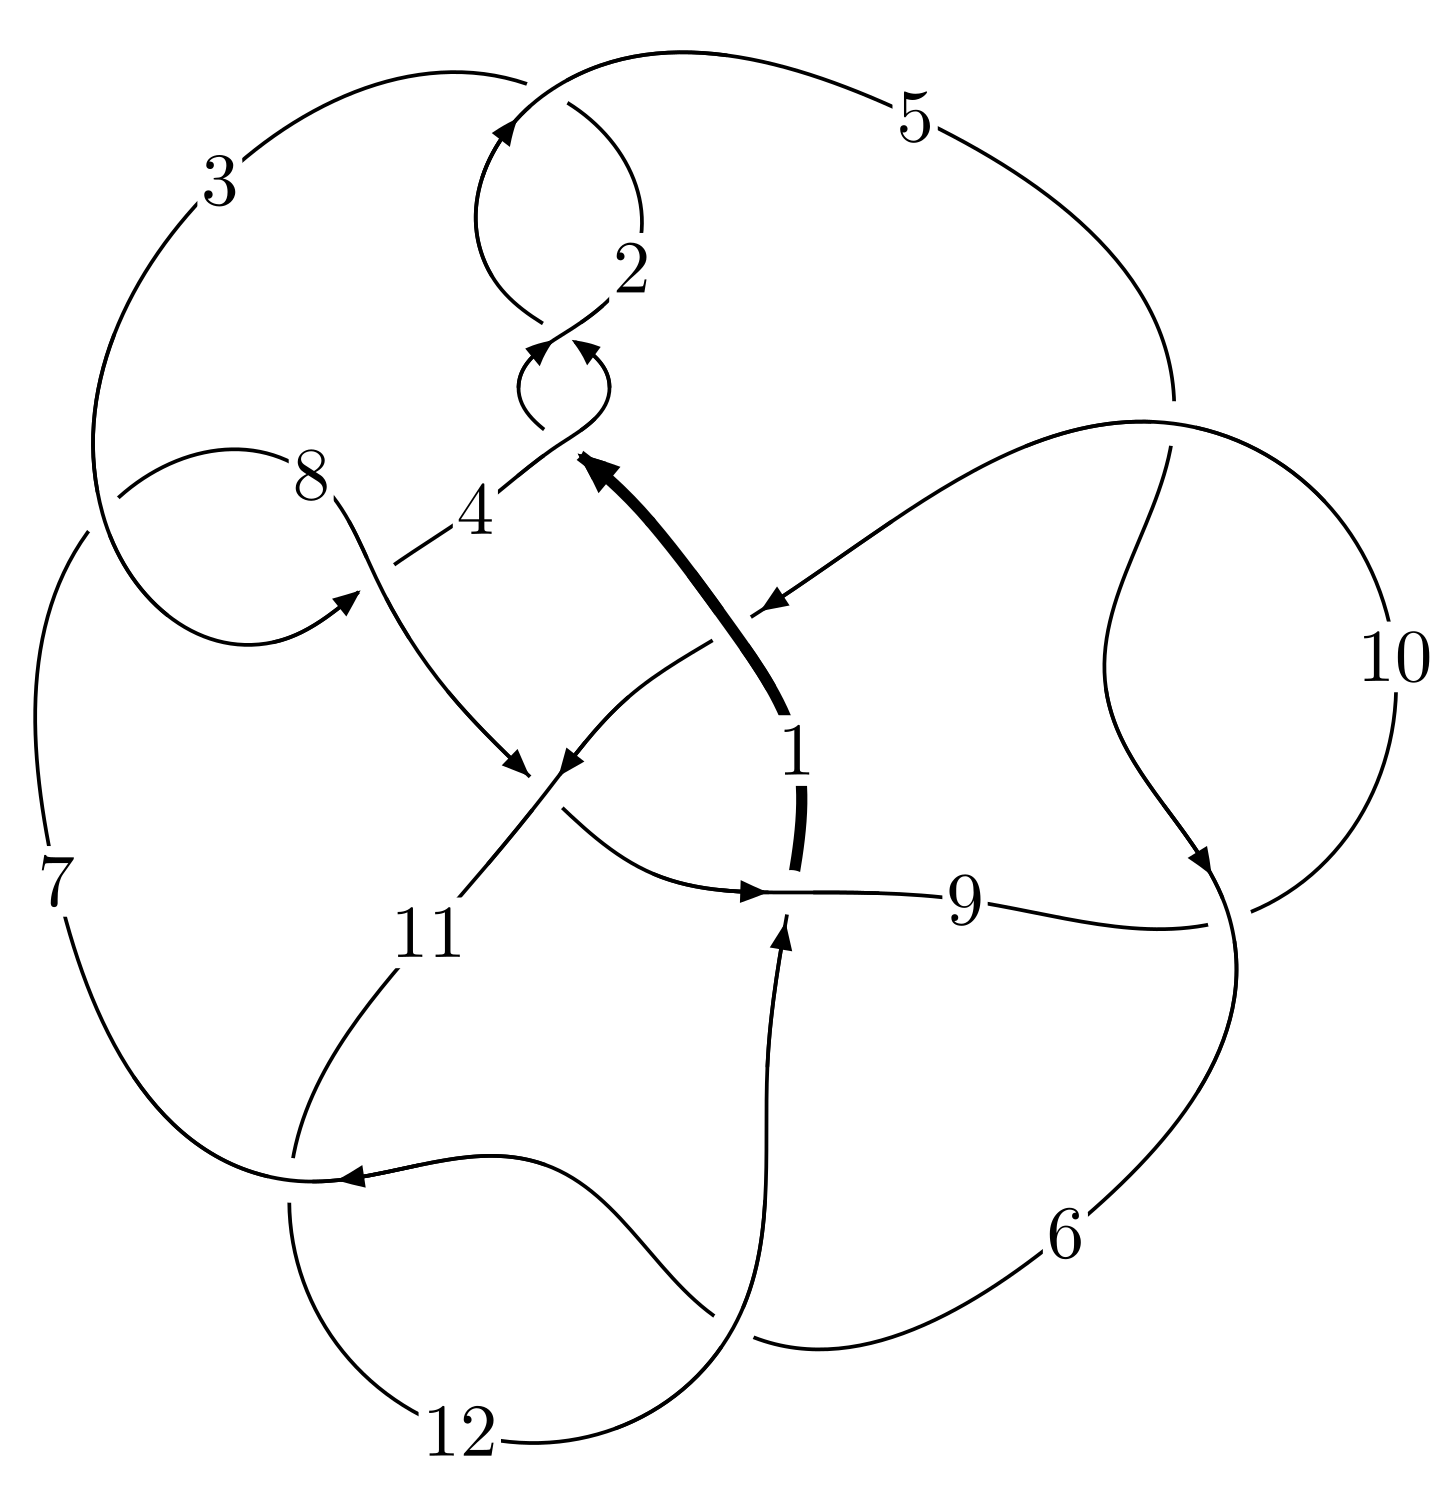
\includegraphics[width=112pt]{../../../GIT/diagram.site/Diagrams/png/1629_12a_0828.png}\\
\ \ \ A knot diagram\footnotemark}&
\allowdisplaybreaks
\textbf{Linearized knot diagam} \\
\cline{2-2}
 &
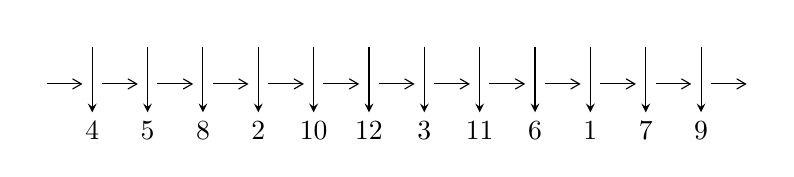
\begin{tikzpicture}[x=20pt, y=17pt]
	% nodes
	\node (C0) at (0, 0) {};
	\node (C1) at (1, 0) {};
	\node (C1U) at (1, +1) {};
	\node (C1D) at (1, -1) {4};

	\node (C2) at (2, 0) {};
	\node (C2U) at (2, +1) {};
	\node (C2D) at (2, -1) {5};

	\node (C3) at (3, 0) {};
	\node (C3U) at (3, +1) {};
	\node (C3D) at (3, -1) {8};

	\node (C4) at (4, 0) {};
	\node (C4U) at (4, +1) {};
	\node (C4D) at (4, -1) {2};

	\node (C5) at (5, 0) {};
	\node (C5U) at (5, +1) {};
	\node (C5D) at (5, -1) {10};

	\node (C6) at (6, 0) {};
	\node (C6U) at (6, +1) {};
	\node (C6D) at (6, -1) {12};

	\node (C7) at (7, 0) {};
	\node (C7U) at (7, +1) {};
	\node (C7D) at (7, -1) {3};

	\node (C8) at (8, 0) {};
	\node (C8U) at (8, +1) {};
	\node (C8D) at (8, -1) {11};

	\node (C9) at (9, 0) {};
	\node (C9U) at (9, +1) {};
	\node (C9D) at (9, -1) {6};

	\node (C10) at (10, 0) {};
	\node (C10U) at (10, +1) {};
	\node (C10D) at (10, -1) {1};

	\node (C11) at (11, 0) {};
	\node (C11U) at (11, +1) {};
	\node (C11D) at (11, -1) {7};

	\node (C12) at (12, 0) {};
	\node (C12U) at (12, +1) {};
	\node (C12D) at (12, -1) {9};
	\node (C13) at (13, 0) {};

	% arrows
	\draw[->,>={angle 60}]
	(C0) edge (C1) (C1) edge (C2) (C2) edge (C3) (C3) edge (C4) (C4) edge (C5) (C5) edge (C6) (C6) edge (C7) (C7) edge (C8) (C8) edge (C9) (C9) edge (C10) (C10) edge (C11) (C11) edge (C12) (C12) edge (C13) ;	\draw[->,>=stealth]
	(C1U) edge (C1D) (C2U) edge (C2D) (C3U) edge (C3D) (C4U) edge (C4D) (C5U) edge (C5D) (C6U) edge (C6D) (C7U) edge (C7D) (C8U) edge (C8D) (C9U) edge (C9D) (C10U) edge (C10D) (C11U) edge (C11D) (C12U) edge (C12D) ;
	\end{tikzpicture} \\
\hhline{~~} \\& 
\textbf{Solving Sequence} \\ \cline{2-2} 
 &
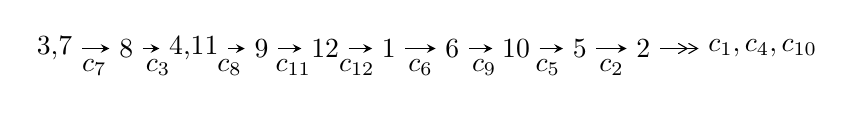
\begin{tikzpicture}[x=23pt, y=7pt]
	% node
	\node (A0) at (-1/8, 0) {3,7};
	\node (A1) at (1, 0) {8};
	\node (A2) at (33/16, 0) {4,11};
	\node (A3) at (25/8, 0) {9};
	\node (A4) at (33/8, 0) {12};
	\node (A5) at (41/8, 0) {1};
	\node (A6) at (49/8, 0) {6};
	\node (A7) at (57/8, 0) {10};
	\node (A8) at (65/8, 0) {5};
	\node (A9) at (73/8, 0) {2};
	\node (C1) at (1/2, -1) {$c_{7}$};
	\node (C2) at (3/2, -1) {$c_{3}$};
	\node (C3) at (21/8, -1) {$c_{8}$};
	\node (C4) at (29/8, -1) {$c_{11}$};
	\node (C5) at (37/8, -1) {$c_{12}$};
	\node (C6) at (45/8, -1) {$c_{6}$};
	\node (C7) at (53/8, -1) {$c_{9}$};
	\node (C8) at (61/8, -1) {$c_{5}$};
	\node (C9) at (69/8, -1) {$c_{2}$};
	\node (A10) at (11, 0) {$c_{1},c_{4},c_{10}$};

	% edge
	\draw[->,>=stealth]	
	(A0) edge (A1) (A1) edge (A2) (A2) edge (A3) (A3) edge (A4) (A4) edge (A5) (A5) edge (A6) (A6) edge (A7) (A7) edge (A8) (A8) edge (A9) ;
	\draw[->>,>={angle 60}]	
	(A9) edge (A10);
\end{tikzpicture} \\ 

\end{tabular} \\

\footnotetext{
The image of knot diagram is generated by the software ``\textbf{Draw programme}" developed by Andrew Bartholomew(\url{http://www.layer8.co.uk/maths/draw/index.htm\#Running-draw}), where we modified some parts for our purpose(\url{https://github.com/CATsTAILs/LinksPainter}).
}\phantom \\ \newline 
\centering \textbf{Ideals for irreducible components\footnotemark of $X_{\text{par}}$} 
 
\begin{align*}
I^u_{1}&=\langle 
1.48295\times10^{68} u^{41}+7.81857\times10^{68} u^{40}+\cdots+7.16827\times10^{67} b-2.61630\times10^{70},\\
\phantom{I^u_{1}}&\phantom{= \langle  }-1.00081\times10^{69} u^{41}-5.50129\times10^{69} u^{40}+\cdots+5.73462\times10^{68} a+2.57458\times10^{71},\\
\phantom{I^u_{1}}&\phantom{= \langle  }u^{42}+6 u^{41}+\cdots-608 u-128\rangle \\
I^u_{2}&=\langle 
46 u^7 a^3-35 u^7 a^2+\cdots+42 a-8,\;6 u^7 a^3+22 u^7 a^2+\cdots-74 a+151,\\
\phantom{I^u_{2}}&\phantom{= \langle  }u^8-3 u^7+3 u^6+2 u^5-8 u^4+9 u^3-3 u^2-2 u+2\rangle \\
I^u_{3}&=\langle 
-2543842 u^{17}-14606334 u^{16}+\cdots+48416059 b+19223447,\\
\phantom{I^u_{3}}&\phantom{= \langle  }-118380102 u^{17}-83676763 u^{16}+\cdots+48416059 a-243963069,\;u^{18}+u^{17}+\cdots+u-1\rangle \\
I^u_{4}&=\langle 
9.40126\times10^{20} a^{7} u^{5}-1.79850\times10^{21} a^{6} u^{5}+\cdots-8.65728\times10^{21} a+3.41117\times10^{21},\\
\phantom{I^u_{4}}&\phantom{= \langle  }-2 a^7 u^5-15 a^6 u^5+\cdots-17 a+4,\;u^6+u^5- u^4-2 u^3+u+1\rangle \\
\\
I^v_{1}&=\langle 
a,\;8 v^2+b+26 v+7,\;4 v^3+14 v^2+7 v+1\rangle \\
I^v_{2}&=\langle 
a,\;b^4+b^3+2 b^2+2 b+1,\;v-1\rangle \\
\end{align*}
\raggedright * 6 irreducible components of $\dim_{\mathbb{C}}=0$, with total 147 representations.\\
\footnotetext{All coefficients of polynomials are rational numbers. But the coefficients are sometimes approximated in decimal forms when there is not enough margin.}
\newpage
\renewcommand{\arraystretch}{1}
\centering \section*{I. $I^u_{1}= \langle 1.48\times10^{68} u^{41}+7.82\times10^{68} u^{40}+\cdots+7.17\times10^{67} b-2.62\times10^{70},\;-1.00\times10^{69} u^{41}-5.50\times10^{69} u^{40}+\cdots+5.73\times10^{68} a+2.57\times10^{71},\;u^{42}+6 u^{41}+\cdots-608 u-128 \rangle$}
\flushleft \textbf{(i) Arc colorings}\\
\begin{tabular}{m{7pt} m{180pt} m{7pt} m{180pt} }
\flushright $a_{3}=$&$\begin{pmatrix}0\\u\end{pmatrix}$ \\
\flushright $a_{7}=$&$\begin{pmatrix}1\\0\end{pmatrix}$ \\
\flushright $a_{8}=$&$\begin{pmatrix}1\\u^2\end{pmatrix}$ \\
\flushright $a_{4}=$&$\begin{pmatrix}- u\\- u^3+u\end{pmatrix}$ \\
\flushright $a_{11}=$&$\begin{pmatrix}1.74520 u^{41}+9.59312 u^{40}+\cdots-1224.97 u-448.953\\-2.06877 u^{41}-10.9072 u^{40}+\cdots+1234.36 u+364.984\end{pmatrix}$ \\
\flushright $a_{9}=$&$\begin{pmatrix}5.46026 u^{41}+28.9099 u^{40}+\cdots-3303.48 u-1037.79\\-0.875191 u^{41}-4.68441 u^{40}+\cdots+555.689 u+190.129\end{pmatrix}$ \\
\flushright $a_{12}=$&$\begin{pmatrix}3.81397 u^{41}+20.5003 u^{40}+\cdots-2459.34 u-813.937\\-2.06877 u^{41}-10.9072 u^{40}+\cdots+1234.36 u+364.984\end{pmatrix}$ \\
\flushright $a_{1}=$&$\begin{pmatrix}-4.29657 u^{41}-22.4006 u^{40}+\cdots+2436.80 u+697.290\\0.303303 u^{41}+1.95238 u^{40}+\cdots-355.882 u-170.418\end{pmatrix}$ \\
\flushright $a_{6}=$&$\begin{pmatrix}-1.88477 u^{41}-9.85936 u^{40}+\cdots+1085.97 u+325.842\\-1.16502 u^{41}-5.92185 u^{40}+\cdots+584.581 u+132.111\end{pmatrix}$ \\
\flushright $a_{10}=$&$\begin{pmatrix}3.30608 u^{41}+17.3565 u^{40}+\cdots-1920.32 u-597.894\\-0.0369235 u^{41}+0.105769 u^{40}+\cdots-130.892 u-62.0948\end{pmatrix}$ \\
\flushright $a_{5}=$&$\begin{pmatrix}-1.33567 u^{41}-6.59646 u^{40}+\cdots+576.521 u+94.3766\\-2.96090 u^{41}-15.8041 u^{40}+\cdots+1860.27 u+602.914\end{pmatrix}$ \\
\flushright $a_{2}=$&$\begin{pmatrix}-3.00789 u^{41}-15.7631 u^{40}+\cdots+1745.87 u+515.839\\-0.0851750 u^{41}-0.0145890 u^{40}+\cdots-165.539 u-129.080\end{pmatrix}$\\&\end{tabular}
\flushleft \textbf{(ii) Obstruction class $= -1$}\\~\\
\flushleft \textbf{(iii) Cusp Shapes $= 50.5421 u^{41}+265.980 u^{40}+\cdots-29786.7 u-9077.56$}\\~\\
\newpage\renewcommand{\arraystretch}{1}
\flushleft \textbf{(iv) u-Polynomials at the component}\newline \\
\begin{tabular}{m{50pt}|m{274pt}}
Crossings & \hspace{64pt}u-Polynomials at each crossing \\
\hline $$\begin{aligned}c_{1},c_{2},c_{4}\end{aligned}$$&$\begin{aligned}
&u^{42}-3 u^{41}+\cdots+140 u+16
\end{aligned}$\\
\hline $$\begin{aligned}c_{3},c_{7}\end{aligned}$$&$\begin{aligned}
&u^{42}-6 u^{41}+\cdots+608 u-128
\end{aligned}$\\
\hline $$\begin{aligned}c_{5},c_{6},c_{9}\\c_{11}\end{aligned}$$&$\begin{aligned}
&u^{42}+16 u^{40}+\cdots+u-1
\end{aligned}$\\
\hline $$\begin{aligned}c_{8},c_{10}\end{aligned}$$&$\begin{aligned}
&u^{42}+2 u^{41}+\cdots+2 u+1
\end{aligned}$\\
\hline $$\begin{aligned}c_{12}\end{aligned}$$&$\begin{aligned}
&u^{42}+39 u^{41}+\cdots+24641536 u+1048576
\end{aligned}$\\
\hline
\end{tabular}\\~\\
\newpage\renewcommand{\arraystretch}{1}
\flushleft \textbf{(v) Riley Polynomials at the component}\newline \\
\begin{tabular}{m{50pt}|m{274pt}}
Crossings & \hspace{64pt}Riley Polynomials at each crossing \\
\hline $$\begin{aligned}c_{1},c_{2},c_{4}\end{aligned}$$&$\begin{aligned}
&y^{42}-37 y^{41}+\cdots-7536 y+256
\end{aligned}$\\
\hline $$\begin{aligned}c_{3},c_{7}\end{aligned}$$&$\begin{aligned}
&y^{42}-18 y^{41}+\cdots-388096 y+16384
\end{aligned}$\\
\hline $$\begin{aligned}c_{5},c_{6},c_{9}\\c_{11}\end{aligned}$$&$\begin{aligned}
&y^{42}+32 y^{41}+\cdots-19 y+1
\end{aligned}$\\
\hline $$\begin{aligned}c_{8},c_{10}\end{aligned}$$&$\begin{aligned}
&y^{42}-2 y^{41}+\cdots-52 y+1
\end{aligned}$\\
\hline $$\begin{aligned}c_{12}\end{aligned}$$&$\begin{aligned}
&y^{42}- y^{41}+\cdots-16217796509696 y+1099511627776
\end{aligned}$\\
\hline
\end{tabular}\\~\\
\newpage\flushleft \textbf{(vi) Complex Volumes and Cusp Shapes}
$$\begin{array}{c|c|c}  
\text{Solutions to }I^u_{1}& \I (\text{vol} + \sqrt{-1}CS) & \text{Cusp shape}\\
 \hline 
\begin{aligned}
u &= \phantom{-}0.943550 + 0.455289 I \\
a &= -1.34280 + 0.76709 I \\
b &= -0.753628 + 0.162890 I\end{aligned}
 & -1.59198 - 3.61998 I & -15.2323 + 5.2048 I \\ \hline\begin{aligned}
u &= \phantom{-}0.943550 - 0.455289 I \\
a &= -1.34280 - 0.76709 I \\
b &= -0.753628 - 0.162890 I\end{aligned}
 & -1.59198 + 3.61998 I & -15.2323 - 5.2048 I \\ \hline\begin{aligned}
u &= -0.269584 + 0.910303 I \\
a &= \phantom{-}0.762837 + 0.613812 I \\
b &= \phantom{-}0.657573 - 0.228220 I\end{aligned}
 & -4.18007 - 1.80472 I & -18.2389 + 0.1966 I \\ \hline\begin{aligned}
u &= -0.269584 - 0.910303 I \\
a &= \phantom{-}0.762837 - 0.613812 I \\
b &= \phantom{-}0.657573 + 0.228220 I\end{aligned}
 & -4.18007 + 1.80472 I & -18.2389 - 0.1966 I \\ \hline\begin{aligned}
u &= \phantom{-}0.062598 + 1.055270 I \\
a &= -0.046684 + 0.319719 I \\
b &= -0.250114 - 1.286520 I\end{aligned}
 & \phantom{-}7.85485 - 3.56337 I & -2.67014 + 3.62743 I \\ \hline\begin{aligned}
u &= \phantom{-}0.062598 - 1.055270 I \\
a &= -0.046684 - 0.319719 I \\
b &= -0.250114 + 1.286520 I\end{aligned}
 & \phantom{-}7.85485 + 3.56337 I & -2.67014 - 3.62743 I \\ \hline\begin{aligned}
u &= \phantom{-}0.466056 + 0.981999 I \\
a &= -0.048754 - 0.335975 I \\
b &= -0.41161 + 1.40369 I\end{aligned}
 & \phantom{-}8.88785 + 7.82161 I & -5.25158 - 5.23582 I \\ \hline\begin{aligned}
u &= \phantom{-}0.466056 - 0.981999 I \\
a &= -0.048754 + 0.335975 I \\
b &= -0.41161 - 1.40369 I\end{aligned}
 & \phantom{-}8.88785 - 7.82161 I & -5.25158 + 5.23582 I \\ \hline\begin{aligned}
u &= -0.786496 + 0.002563 I \\
a &= -2.39632 + 0.05081 I \\
b &= -0.465074 - 0.281780 I\end{aligned}
 & -2.91939 - 0.16667 I & -21.2268 + 8.1932 I \\ \hline\begin{aligned}
u &= -0.786496 - 0.002563 I \\
a &= -2.39632 - 0.05081 I \\
b &= -0.465074 + 0.281780 I\end{aligned}
 & -2.91939 + 0.16667 I & -21.2268 - 8.1932 I\\
 \hline 
 \end{array}$$\newpage$$\begin{array}{c|c|c}  
\text{Solutions to }I^u_{1}& \I (\text{vol} + \sqrt{-1}CS) & \text{Cusp shape}\\
 \hline 
\begin{aligned}
u &= -1.184420 + 0.429182 I \\
a &= \phantom{-}0.697295 + 0.202000 I \\
b &= \phantom{-}0.812246 + 0.378376 I\end{aligned}
 & -5.91413 + 2.39057 I & \phantom{-0.000000 } 0 \\ \hline\begin{aligned}
u &= -1.184420 - 0.429182 I \\
a &= \phantom{-}0.697295 - 0.202000 I \\
b &= \phantom{-}0.812246 - 0.378376 I\end{aligned}
 & -5.91413 - 2.39057 I & \phantom{-0.000000 } 0 \\ \hline\begin{aligned}
u &= \phantom{-}1.253720 + 0.213033 I \\
a &= -1.287820 + 0.268400 I \\
b &= -0.606517 - 0.635131 I\end{aligned}
 & -9.38202 - 1.73644 I & \phantom{-0.000000 } 0 \\ \hline\begin{aligned}
u &= \phantom{-}1.253720 - 0.213033 I \\
a &= -1.287820 - 0.268400 I \\
b &= -0.606517 + 0.635131 I\end{aligned}
 & -9.38202 + 1.73644 I & \phantom{-0.000000 } 0 \\ \hline\begin{aligned}
u &= -1.171280 + 0.521960 I \\
a &= \phantom{-}1.69502 - 0.32871 I \\
b &= \phantom{-}0.49391 - 1.37449 I\end{aligned}
 & \phantom{-}4.28505 + 8.46529 I & \phantom{-0.000000 } 0 \\ \hline\begin{aligned}
u &= -1.171280 - 0.521960 I \\
a &= \phantom{-}1.69502 + 0.32871 I \\
b &= \phantom{-}0.49391 + 1.37449 I\end{aligned}
 & \phantom{-}4.28505 - 8.46529 I & \phantom{-0.000000 } 0 \\ \hline\begin{aligned}
u &= -1.183490 + 0.564393 I \\
a &= -1.075040 - 0.521185 I \\
b &= -0.905363 - 0.213820 I\end{aligned}
 & -7.00695 + 7.14218 I & \phantom{-0.000000 } 0 \\ \hline\begin{aligned}
u &= -1.183490 - 0.564393 I \\
a &= -1.075040 + 0.521185 I \\
b &= -0.905363 + 0.213820 I\end{aligned}
 & -7.00695 - 7.14218 I & \phantom{-0.000000 } 0 \\ \hline\begin{aligned}
u &= \phantom{-}0.582949 + 0.315976 I \\
a &= \phantom{-}0.876169 - 0.195926 I \\
b &= \phantom{-}0.539552 - 0.112152 I\end{aligned}
 & -0.538615 - 0.005437 I & -12.84477 - 0.43346 I \\ \hline\begin{aligned}
u &= \phantom{-}0.582949 - 0.315976 I \\
a &= \phantom{-}0.876169 + 0.195926 I \\
b &= \phantom{-}0.539552 + 0.112152 I\end{aligned}
 & -0.538615 + 0.005437 I & -12.84477 + 0.43346 I\\
 \hline 
 \end{array}$$\newpage$$\begin{array}{c|c|c}  
\text{Solutions to }I^u_{1}& \I (\text{vol} + \sqrt{-1}CS) & \text{Cusp shape}\\
 \hline 
\begin{aligned}
u &= -0.610840 + 1.193460 I \\
a &= -0.054193 + 0.342180 I \\
b &= -0.52479 - 1.40750 I\end{aligned}
 & \phantom{-}3.43638 - 11.55830 I & \phantom{-0.000000 } 0 \\ \hline\begin{aligned}
u &= -0.610840 - 1.193460 I \\
a &= -0.054193 - 0.342180 I \\
b &= -0.52479 + 1.40750 I\end{aligned}
 & \phantom{-}3.43638 + 11.55830 I & \phantom{-0.000000 } 0 \\ \hline\begin{aligned}
u &= \phantom{-}1.163520 + 0.689411 I \\
a &= \phantom{-}1.72107 - 0.08499 I \\
b &= \phantom{-}0.52703 + 1.44729 I\end{aligned}
 & \phantom{-}6.7272 - 13.9058 I & \phantom{-0.000000 } 0 \\ \hline\begin{aligned}
u &= \phantom{-}1.163520 - 0.689411 I \\
a &= \phantom{-}1.72107 + 0.08499 I \\
b &= \phantom{-}0.52703 - 1.44729 I\end{aligned}
 & \phantom{-}6.7272 + 13.9058 I & \phantom{-0.000000 } 0 \\ \hline\begin{aligned}
u &= \phantom{-}0.534889 + 1.254550 I \\
a &= \phantom{-}0.262606 - 0.299605 I \\
b &= -0.206473 + 0.740584 I\end{aligned}
 & -1.23399 + 1.54080 I & \phantom{-0.000000 } 0 \\ \hline\begin{aligned}
u &= \phantom{-}0.534889 - 1.254550 I \\
a &= \phantom{-}0.262606 + 0.299605 I \\
b &= -0.206473 - 0.740584 I\end{aligned}
 & -1.23399 - 1.54080 I & \phantom{-0.000000 } 0 \\ \hline\begin{aligned}
u &= -0.535582 + 0.088545 I \\
a &= -0.050104 + 0.333280 I \\
b &= -0.22875 - 1.51299 I\end{aligned}
 & \phantom{-}7.50056 - 5.01376 I & -21.5440 - 1.4253 I \\ \hline\begin{aligned}
u &= -0.535582 - 0.088545 I \\
a &= -0.050104 - 0.333280 I \\
b &= -0.22875 + 1.51299 I\end{aligned}
 & \phantom{-}7.50056 + 5.01376 I & -21.5440 + 1.4253 I \\ \hline\begin{aligned}
u &= -1.22163 + 0.80316 I \\
a &= \phantom{-}1.55023 + 0.27538 I \\
b &= \phantom{-}0.56950 - 1.48815 I\end{aligned}
 & \phantom{-}1.4008 + 18.6869 I & \phantom{-0.000000 } 0 \\ \hline\begin{aligned}
u &= -1.22163 - 0.80316 I \\
a &= \phantom{-}1.55023 - 0.27538 I \\
b &= \phantom{-}0.56950 + 1.48815 I\end{aligned}
 & \phantom{-}1.4008 - 18.6869 I & \phantom{-0.000000 } 0\\
 \hline 
 \end{array}$$\newpage$$\begin{array}{c|c|c}  
\text{Solutions to }I^u_{1}& \I (\text{vol} + \sqrt{-1}CS) & \text{Cusp shape}\\
 \hline 
\begin{aligned}
u &= -1.17869 + 0.90581 I \\
a &= -0.942618 - 0.308680 I \\
b &= -0.163308 + 1.189210 I\end{aligned}
 & -0.91717 + 9.50337 I & \phantom{-0.000000 } 0 \\ \hline\begin{aligned}
u &= -1.17869 - 0.90581 I \\
a &= -0.942618 + 0.308680 I \\
b &= -0.163308 - 1.189210 I\end{aligned}
 & -0.91717 - 9.50337 I & \phantom{-0.000000 } 0 \\ \hline\begin{aligned}
u &= -0.491641\phantom{ +0.000000I} \\
a &= -4.91091\phantom{ +0.000000I} \\
b &= -0.343981\phantom{ +0.000000I}\end{aligned}
 & -2.80521\phantom{ +0.000000I} & -47.0160\phantom{ +0.000000I} \\ \hline\begin{aligned}
u &= \phantom{-}1.20729 + 0.91942 I \\
a &= -0.752800 + 0.170890 I \\
b &= -0.065111 - 1.139040 I\end{aligned}
 & \phantom{-}4.02842 - 4.18037 I & \phantom{-0.000000 } 0 \\ \hline\begin{aligned}
u &= \phantom{-}1.20729 - 0.91942 I \\
a &= -0.752800 - 0.170890 I \\
b &= -0.065111 + 1.139040 I\end{aligned}
 & \phantom{-}4.02842 + 4.18037 I & \phantom{-0.000000 } 0 \\ \hline\begin{aligned}
u &= \phantom{-}1.48911 + 0.29406 I \\
a &= \phantom{-}0.896680 + 0.297454 I \\
b &= \phantom{-}0.617444 + 1.108590 I\end{aligned}
 & -6.18728 - 8.08758 I & \phantom{-0.000000 } 0 \\ \hline\begin{aligned}
u &= \phantom{-}1.48911 - 0.29406 I \\
a &= \phantom{-}0.896680 - 0.297454 I \\
b &= \phantom{-}0.617444 - 1.108590 I\end{aligned}
 & -6.18728 + 8.08758 I & \phantom{-0.000000 } 0 \\ \hline\begin{aligned}
u &= -1.50353 + 0.22766 I \\
a &= \phantom{-}0.444601 - 0.413741 I \\
b &= \phantom{-}0.308344 - 0.976227 I\end{aligned}
 & \phantom{-}1.53844 + 4.49579 I & \phantom{-0.000000 } 0 \\ \hline\begin{aligned}
u &= -1.50353 - 0.22766 I \\
a &= \phantom{-}0.444601 + 0.413741 I \\
b &= \phantom{-}0.308344 + 0.976227 I\end{aligned}
 & \phantom{-}1.53844 - 4.49579 I & \phantom{-0.000000 } 0 \\ \hline\begin{aligned}
u &= -1.01992 + 1.13548 I \\
a &= -0.362994 - 0.380675 I \\
b &= \phantom{-}0.031656 + 1.071510 I\end{aligned}
 & \phantom{-}0.04635 - 1.77468 I & \phantom{-0.000000 } 0\\
 \hline 
 \end{array}$$\newpage$$\begin{array}{c|c|c}  
\text{Solutions to }I^u_{1}& \I (\text{vol} + \sqrt{-1}CS) & \text{Cusp shape}\\
 \hline 
\begin{aligned}
u &= -1.01992 - 1.13548 I \\
a &= -0.362994 + 0.380675 I \\
b &= \phantom{-}0.031656 - 1.071510 I\end{aligned}
 & \phantom{-}0.04635 + 1.77468 I & \phantom{-0.000000 } 0 \\ \hline\begin{aligned}
u &= \phantom{-}0.415199\phantom{ +0.000000I} \\
a &= \phantom{-}0.943147\phantom{ +0.000000I} \\
b &= \phantom{-}0.390970\phantom{ +0.000000I}\end{aligned}
 & -0.638593\phantom{ +0.000000I} & -15.1720\phantom{ +0.000000I}\\
 \hline 
 \end{array}$$\newpage\newpage\renewcommand{\arraystretch}{1}
\centering \section*{II. $I^u_{2}= \langle 46 u^7 a^3-35 u^7 a^2+\cdots+42 a-8,\;6 u^7 a^3+22 u^7 a^2+\cdots-74 a+151,\;u^8-3 u^7+\cdots-2 u+2 \rangle$}
\flushleft \textbf{(i) Arc colorings}\\
\begin{tabular}{m{7pt} m{180pt} m{7pt} m{180pt} }
\flushright $a_{3}=$&$\begin{pmatrix}0\\u\end{pmatrix}$ \\
\flushright $a_{7}=$&$\begin{pmatrix}1\\0\end{pmatrix}$ \\
\flushright $a_{8}=$&$\begin{pmatrix}1\\u^2\end{pmatrix}$ \\
\flushright $a_{4}=$&$\begin{pmatrix}- u\\- u^3+u\end{pmatrix}$ \\
\flushright $a_{11}=$&$\begin{pmatrix}a\\-1.58621 a^{3} u^{7}+1.20690 a^{2} u^{7}+\cdots-1.44828 a+0.275862\end{pmatrix}$ \\
\flushright $a_{9}=$&$\begin{pmatrix}-0.793103 a^{3} u^{7}+0.206897 a^{2} u^{7}+\cdots+0.275862 a-5.72414\\-0.206897 a^{2} u^{7}-0.896552 u^{7}+\cdots+0.551724 a^{2}-0.275862\end{pmatrix}$ \\
\flushright $a_{12}=$&$\begin{pmatrix}1.58621 a^{3} u^{7}-1.20690 a^{2} u^{7}+\cdots+2.44828 a-0.275862\\-1.58621 a^{3} u^{7}+1.20690 a^{2} u^{7}+\cdots-1.44828 a+0.275862\end{pmatrix}$ \\
\flushright $a_{1}=$&$\begin{pmatrix}\frac{3}{2} u^7-\frac{7}{2} u^6+\cdots+\frac{3}{2} u-3\\- u^7+2 u^6- u^5-3 u^4+5 u^3-3 u^2- u+1\end{pmatrix}$ \\
\flushright $a_{6}=$&$\begin{pmatrix}1.03448 a^{3} u^{7}-1.17241 a^{2} u^{7}+\cdots-4.62069 a+5.10345\\-0.241379 a^{3} u^{7}+0.965517 a^{2} u^{7}+\cdots+4.34483 a+2.62069\end{pmatrix}$ \\
\flushright $a_{10}=$&$\begin{pmatrix}-1.58621 a^{3} u^{7}+1.20690 a^{2} u^{7}+\cdots+3.55172 a-5.72414\\0.586207 a^{3} u^{7}-0.206897 a^{2} u^{7}+\cdots-4.55172 a+2.72414\end{pmatrix}$ \\
\flushright $a_{5}=$&$\begin{pmatrix}\frac{1}{2} u^7-\frac{1}{2} u^6+\cdots-\frac{1}{2} u^2+\frac{3}{2} u\\u^7-3 u^6+2 u^5+3 u^4-8 u^3+6 u^2-3\end{pmatrix}$ \\
\flushright $a_{2}=$&$\begin{pmatrix}\frac{1}{2} u^7-\frac{3}{2} u^6+\cdots+\frac{1}{2} u-1\\- u^7+2 u^6-3 u^4+4 u^3-2 u^2+1\end{pmatrix}$\\&\end{tabular}
\flushleft \textbf{(ii) Obstruction class $= -1$}\\~\\
\flushleft \textbf{(iii) Cusp Shapes $= -\frac{48}{29} u^7 a^3+\frac{92}{29} u^7 a^2+\cdots-\frac{64}{29} a-\frac{264}{29}$}\\~\\
\newpage\renewcommand{\arraystretch}{1}
\flushleft \textbf{(iv) u-Polynomials at the component}\newline \\
\begin{tabular}{m{50pt}|m{274pt}}
Crossings & \hspace{64pt}u-Polynomials at each crossing \\
\hline $$\begin{aligned}c_{1},c_{2},c_{4}\end{aligned}$$&$\begin{aligned}
&(u^8- u^7-4 u^6+3 u^5+5 u^4- u^3- u^2-3 u-1)^4
\end{aligned}$\\
\hline $$\begin{aligned}c_{3},c_{7}\end{aligned}$$&$\begin{aligned}
&(u^8+3 u^7+3 u^6-2 u^5-8 u^4-9 u^3-3 u^2+2 u+2)^4
\end{aligned}$\\
\hline $$\begin{aligned}c_{5},c_{6},c_{9}\\c_{11}\end{aligned}$$&$\begin{aligned}
&u^{32}+u^{31}+\cdots-108 u+19
\end{aligned}$\\
\hline $$\begin{aligned}c_{8},c_{10}\end{aligned}$$&$\begin{aligned}
&u^{32}-7 u^{31}+\cdots-148 u+13
\end{aligned}$\\
\hline $$\begin{aligned}c_{12}\end{aligned}$$&$\begin{aligned}
&(u^2- u+1)^{16}
\end{aligned}$\\
\hline
\end{tabular}\\~\\
\newpage\renewcommand{\arraystretch}{1}
\flushleft \textbf{(v) Riley Polynomials at the component}\newline \\
\begin{tabular}{m{50pt}|m{274pt}}
Crossings & \hspace{64pt}Riley Polynomials at each crossing \\
\hline $$\begin{aligned}c_{1},c_{2},c_{4}\end{aligned}$$&$\begin{aligned}
&(y^8-9 y^7+32 y^6-53 y^5+31 y^4+15 y^3-15 y^2-7 y+1)^4
\end{aligned}$\\
\hline $$\begin{aligned}c_{3},c_{7}\end{aligned}$$&$\begin{aligned}
&(y^8-3 y^7+5 y^6-4 y^5+2 y^4-13 y^3+13 y^2-16 y+4)^4
\end{aligned}$\\
\hline $$\begin{aligned}c_{5},c_{6},c_{9}\\c_{11}\end{aligned}$$&$\begin{aligned}
&y^{32}+21 y^{31}+\cdots+6120 y+361
\end{aligned}$\\
\hline $$\begin{aligned}c_{8},c_{10}\end{aligned}$$&$\begin{aligned}
&y^{32}+y^{31}+\cdots+248 y+169
\end{aligned}$\\
\hline $$\begin{aligned}c_{12}\end{aligned}$$&$\begin{aligned}
&(y^2+y+1)^{16}
\end{aligned}$\\
\hline
\end{tabular}\\~\\
\newpage\flushleft \textbf{(vi) Complex Volumes and Cusp Shapes}
$$\begin{array}{c|c|c}  
\text{Solutions to }I^u_{2}& \I (\text{vol} + \sqrt{-1}CS) & \text{Cusp shape}\\
 \hline 
\begin{aligned}
u &= \phantom{-}0.821613 + 0.567011 I \\
a &= -0.496625 - 0.438250 I \\
b &= \phantom{-}0.52992 - 1.64688 I\end{aligned}
 & \phantom{-}6.41985 - 0.23387 I & -3.94128 + 1.06967 I \\ \hline\begin{aligned}
u &= \phantom{-}0.821613 + 0.567011 I \\
a &= \phantom{-}0.26645 - 1.48983 I \\
b &= \phantom{-}0.073416 + 1.309500 I\end{aligned}
 & \phantom{-}6.41985 - 4.29364 I & -3.94128 + 7.99788 I \\ \hline\begin{aligned}
u &= \phantom{-}0.821613 + 0.567011 I \\
a &= -2.39394 + 0.27463 I \\
b &= -0.73198 - 1.51497 I\end{aligned}
 & \phantom{-}6.41985 - 4.29364 I & -3.94128 + 7.99788 I \\ \hline\begin{aligned}
u &= \phantom{-}0.821613 + 0.567011 I \\
a &= \phantom{-}2.61276 - 0.79661 I \\
b &= -0.022697 + 1.179290 I\end{aligned}
 & \phantom{-}6.41985 - 0.23387 I & -3.94128 + 1.06967 I \\ \hline\begin{aligned}
u &= \phantom{-}0.821613 - 0.567011 I \\
a &= -0.496625 + 0.438250 I \\
b &= \phantom{-}0.52992 + 1.64688 I\end{aligned}
 & \phantom{-}6.41985 + 0.23387 I & -3.94128 - 1.06967 I \\ \hline\begin{aligned}
u &= \phantom{-}0.821613 - 0.567011 I \\
a &= \phantom{-}0.26645 + 1.48983 I \\
b &= \phantom{-}0.073416 - 1.309500 I\end{aligned}
 & \phantom{-}6.41985 + 4.29364 I & -3.94128 - 7.99788 I \\ \hline\begin{aligned}
u &= \phantom{-}0.821613 - 0.567011 I \\
a &= -2.39394 - 0.27463 I \\
b &= -0.73198 + 1.51497 I\end{aligned}
 & \phantom{-}6.41985 + 4.29364 I & -3.94128 - 7.99788 I \\ \hline\begin{aligned}
u &= \phantom{-}0.821613 - 0.567011 I \\
a &= \phantom{-}2.61276 + 0.79661 I \\
b &= -0.022697 - 1.179290 I\end{aligned}
 & \phantom{-}6.41985 + 0.23387 I & -3.94128 - 1.06967 I \\ \hline\begin{aligned}
u &= \phantom{-}0.432344 + 1.079150 I \\
a &= -0.100401 + 0.617152 I \\
b &= -1.201190 + 0.090721 I\end{aligned}
 & -1.29038 + 5.58743 I & -12.52739 - 6.08899 I \\ \hline\begin{aligned}
u &= \phantom{-}0.432344 + 1.079150 I \\
a &= \phantom{-}0.361262 - 0.454625 I \\
b &= -0.207449 + 0.429798 I\end{aligned}
 & -1.29038 + 1.52767 I & -12.52739 + 0.83921 I\\
 \hline 
 \end{array}$$\newpage$$\begin{array}{c|c|c}  
\text{Solutions to }I^u_{2}& \I (\text{vol} + \sqrt{-1}CS) & \text{Cusp shape}\\
 \hline 
\begin{aligned}
u &= \phantom{-}0.432344 + 1.079150 I \\
a &= \phantom{-}0.451119 + 0.354898 I \\
b &= \phantom{-}0.341939 - 1.164380 I\end{aligned}
 & -1.29038 + 5.58743 I & -12.52739 - 6.08899 I \\ \hline\begin{aligned}
u &= \phantom{-}0.432344 + 1.079150 I \\
a &= \phantom{-}0.305199 - 0.335131 I \\
b &= -0.292741 + 0.851162 I\end{aligned}
 & -1.29038 + 1.52767 I & -12.52739 + 0.83921 I \\ \hline\begin{aligned}
u &= \phantom{-}0.432344 - 1.079150 I \\
a &= -0.100401 - 0.617152 I \\
b &= -1.201190 - 0.090721 I\end{aligned}
 & -1.29038 - 5.58743 I & -12.52739 + 6.08899 I \\ \hline\begin{aligned}
u &= \phantom{-}0.432344 - 1.079150 I \\
a &= \phantom{-}0.361262 + 0.454625 I \\
b &= -0.207449 - 0.429798 I\end{aligned}
 & -1.29038 - 1.52767 I & -12.52739 - 0.83921 I \\ \hline\begin{aligned}
u &= \phantom{-}0.432344 - 1.079150 I \\
a &= \phantom{-}0.451119 - 0.354898 I \\
b &= \phantom{-}0.341939 + 1.164380 I\end{aligned}
 & -1.29038 - 5.58743 I & -12.52739 + 6.08899 I \\ \hline\begin{aligned}
u &= \phantom{-}0.432344 - 1.079150 I \\
a &= \phantom{-}0.305199 + 0.335131 I \\
b &= -0.292741 - 0.851162 I\end{aligned}
 & -1.29038 - 1.52767 I & -12.52739 - 0.83921 I \\ \hline\begin{aligned}
u &= -1.38845\phantom{ +0.000000I} \\
a &= -0.810223 + 0.602331 I \\
b &= -0.367950 + 0.903689 I\end{aligned}
 & -8.50968 + 2.02988 I & -16.3375 - 3.4641 I \\ \hline\begin{aligned}
u &= -1.38845\phantom{ +0.000000I} \\
a &= -0.810223 - 0.602331 I \\
b &= -0.367950 - 0.903689 I\end{aligned}
 & -8.50968 - 2.02988 I & -16.3375 + 3.4641 I \\ \hline\begin{aligned}
u &= -1.38845\phantom{ +0.000000I} \\
a &= \phantom{-}1.129680 + 0.049021 I \\
b &= \phantom{-}1.122510 - 0.403244 I\end{aligned}
 & -8.50968 - 2.02988 I & -16.3375 + 3.4641 I \\ \hline\begin{aligned}
u &= -1.38845\phantom{ +0.000000I} \\
a &= \phantom{-}1.129680 - 0.049021 I \\
b &= \phantom{-}1.122510 + 0.403244 I\end{aligned}
 & -8.50968 + 2.02988 I & -16.3375 - 3.4641 I\\
 \hline 
 \end{array}$$\newpage$$\begin{array}{c|c|c}  
\text{Solutions to }I^u_{2}& \I (\text{vol} + \sqrt{-1}CS) & \text{Cusp shape}\\
 \hline 
\begin{aligned}
u &= \phantom{-}1.215250 + 0.684012 I \\
a &= \phantom{-}1.165160 - 0.211690 I \\
b &= \phantom{-}0.639095 + 1.148790 I\end{aligned}
 & -3.80498 - 7.85312 I & -13.28252 + 2.60552 I \\ \hline\begin{aligned}
u &= \phantom{-}1.215250 + 0.684012 I \\
a &= \phantom{-}1.086450 - 0.626118 I \\
b &= \phantom{-}1.43070 + 0.15248 I\end{aligned}
 & -3.80498 - 11.91290 I & -13.2825 + 9.5337 I \\ \hline\begin{aligned}
u &= \phantom{-}1.215250 + 0.684012 I \\
a &= -0.387082 - 0.088325 I \\
b &= -0.213058 + 0.253663 I\end{aligned}
 & -3.80498 - 7.85312 I & -13.28252 + 2.60552 I \\ \hline\begin{aligned}
u &= \phantom{-}1.215250 + 0.684012 I \\
a &= -1.73531 + 0.10229 I \\
b &= -0.429159 - 1.222660 I\end{aligned}
 & -3.80498 - 11.91290 I & -13.2825 + 9.5337 I \\ \hline\begin{aligned}
u &= \phantom{-}1.215250 - 0.684012 I \\
a &= \phantom{-}1.165160 + 0.211690 I \\
b &= \phantom{-}0.639095 - 1.148790 I\end{aligned}
 & -3.80498 + 7.85312 I & -13.28252 - 2.60552 I \\ \hline\begin{aligned}
u &= \phantom{-}1.215250 - 0.684012 I \\
a &= \phantom{-}1.086450 + 0.626118 I \\
b &= \phantom{-}1.43070 - 0.15248 I\end{aligned}
 & -3.80498 + 11.91290 I & -13.2825 - 9.5337 I \\ \hline\begin{aligned}
u &= \phantom{-}1.215250 - 0.684012 I \\
a &= -0.387082 + 0.088325 I \\
b &= -0.213058 - 0.253663 I\end{aligned}
 & -3.80498 + 7.85312 I & -13.28252 - 2.60552 I \\ \hline\begin{aligned}
u &= \phantom{-}1.215250 - 0.684012 I \\
a &= -1.73531 - 0.10229 I \\
b &= -0.429159 + 1.222660 I\end{aligned}
 & -3.80498 + 11.91290 I & -13.2825 - 9.5337 I \\ \hline\begin{aligned}
u &= -0.549965\phantom{ +0.000000I} \\
a &= \phantom{-}2.01507 + 0.46937 I \\
b &= \phantom{-}0.255913 + 1.378810 I\end{aligned}
 & \phantom{-}4.21577 - 2.02988 I & -12.16015 + 3.46410 I \\ \hline\begin{aligned}
u &= -0.549965\phantom{ +0.000000I} \\
a &= \phantom{-}2.01507 - 0.46937 I \\
b &= \phantom{-}0.255913 - 1.378810 I\end{aligned}
 & \phantom{-}4.21577 + 2.02988 I & -12.16015 - 3.46410 I\\
 \hline 
 \end{array}$$\newpage$$\begin{array}{c|c|c}  
\text{Solutions to }I^u_{2}& \I (\text{vol} + \sqrt{-1}CS) & \text{Cusp shape}\\
 \hline 
\begin{aligned}
u &= -0.549965\phantom{ +0.000000I} \\
a &= \phantom{-}0.53043 + 4.87830 I \\
b &= -0.427270 + 1.082010 I\end{aligned}
 & \phantom{-}4.21577 + 2.02988 I & -12.16015 - 3.46410 I \\ \hline\begin{aligned}
u &= -0.549965\phantom{ +0.000000I} \\
a &= \phantom{-}0.53043 - 4.87830 I \\
b &= -0.427270 - 1.082010 I\end{aligned}
 & \phantom{-}4.21577 - 2.02988 I & -12.16015 + 3.46410 I\\
 \hline 
 \end{array}$$\newpage\newpage\renewcommand{\arraystretch}{1}
\centering \section*{III. $I^u_{3}= \langle -2.54\times10^{6} u^{17}-1.46\times10^{7} u^{16}+\cdots+4.84\times10^{7} b+1.92\times10^{7},\;-1.18\times10^{8} u^{17}-8.37\times10^{7} u^{16}+\cdots+4.84\times10^{7} a-2.44\times10^{8},\;u^{18}+u^{17}+\cdots+u-1 \rangle$}
\flushleft \textbf{(i) Arc colorings}\\
\begin{tabular}{m{7pt} m{180pt} m{7pt} m{180pt} }
\flushright $a_{3}=$&$\begin{pmatrix}0\\u\end{pmatrix}$ \\
\flushright $a_{7}=$&$\begin{pmatrix}1\\0\end{pmatrix}$ \\
\flushright $a_{8}=$&$\begin{pmatrix}1\\u^2\end{pmatrix}$ \\
\flushright $a_{4}=$&$\begin{pmatrix}- u\\- u^3+u\end{pmatrix}$ \\
\flushright $a_{11}=$&$\begin{pmatrix}2.44506 u^{17}+1.72829 u^{16}+\cdots-2.56183 u+5.03889\\0.0525413 u^{17}+0.301684 u^{16}+\cdots+0.880761 u-0.397047\end{pmatrix}$ \\
\flushright $a_{9}=$&$\begin{pmatrix}0.999862 u^{17}+1.73119 u^{16}+\cdots-5.39506 u-5.34506\\-0.411438 u^{17}-0.578846 u^{16}+\cdots+0.180593 u+0.176599\end{pmatrix}$ \\
\flushright $a_{12}=$&$\begin{pmatrix}2.39252 u^{17}+1.42660 u^{16}+\cdots-3.44259 u+5.43593\\0.0525413 u^{17}+0.301684 u^{16}+\cdots+0.880761 u-0.397047\end{pmatrix}$ \\
\flushright $a_{1}=$&$\begin{pmatrix}0.482663 u^{17}+0.187223 u^{16}+\cdots-0.596217 u+0.702631\\0.0998597 u^{17}+0.114275 u^{16}+\cdots+0.581502 u-0.0462974\end{pmatrix}$ \\
\flushright $a_{6}=$&$\begin{pmatrix}3.34248 u^{17}+4.59289 u^{16}+\cdots-17.7756 u+0.849286\\-0.0239398 u^{17}-0.417477 u^{16}+\cdots+2.28107 u+0.680274\end{pmatrix}$ \\
\flushright $a_{10}=$&$\begin{pmatrix}2.03362 u^{17}+1.14944 u^{16}+\cdots-2.38124 u+6.21549\\0.0525413 u^{17}+0.301684 u^{16}+\cdots+0.880761 u-0.397047\end{pmatrix}$ \\
\flushright $a_{5}=$&$\begin{pmatrix}-0.602448 u^{17}-0.364456 u^{16}+\cdots+0.792818 u-0.951774\\0.119785 u^{17}+0.177233 u^{16}+\cdots-0.196601 u+0.249142\end{pmatrix}$ \\
\flushright $a_{2}=$&$\begin{pmatrix}0.527854 u^{17}+0.454267 u^{16}+\cdots-1.43666 u+0.940623\\-0.0332079 u^{17}-0.113318 u^{16}+\cdots+1.24528 u-0.0624363\end{pmatrix}$\\&\end{tabular}
\flushleft \textbf{(ii) Obstruction class $= 1$}\\~\\
\flushleft \textbf{(iii) Cusp Shapes $= -\frac{191549447}{48416059} u^{17}-\frac{183440518}{48416059} u^{16}+\cdots+\frac{478561907}{48416059} u-\frac{255825818}{48416059}$}\\~\\
\newpage\renewcommand{\arraystretch}{1}
\flushleft \textbf{(iv) u-Polynomials at the component}\newline \\
\begin{tabular}{m{50pt}|m{274pt}}
Crossings & \hspace{64pt}u-Polynomials at each crossing \\
\hline $$\begin{aligned}c_{1},c_{2}\end{aligned}$$&$\begin{aligned}
&u^{18}+3 u^{17}+\cdots+3 u-1
\end{aligned}$\\
\hline $$\begin{aligned}c_{3}\end{aligned}$$&$\begin{aligned}
&u^{18}- u^{17}+\cdots- u-1
\end{aligned}$\\
\hline $$\begin{aligned}c_{4}\end{aligned}$$&$\begin{aligned}
&u^{18}-3 u^{17}+\cdots-3 u-1
\end{aligned}$\\
\hline $$\begin{aligned}c_{5},c_{11}\end{aligned}$$&$\begin{aligned}
&u^{18}+10 u^{16}+\cdots-10 u+1
\end{aligned}$\\
\hline $$\begin{aligned}c_{6},c_{9}\end{aligned}$$&$\begin{aligned}
&u^{18}+10 u^{16}+\cdots+10 u+1
\end{aligned}$\\
\hline $$\begin{aligned}c_{7}\end{aligned}$$&$\begin{aligned}
&u^{18}+u^{17}+\cdots+u-1
\end{aligned}$\\
\hline $$\begin{aligned}c_{8},c_{10}\end{aligned}$$&$\begin{aligned}
&u^{18}+2 u^{17}+\cdots-3 u+1
\end{aligned}$\\
\hline $$\begin{aligned}c_{12}\end{aligned}$$&$\begin{aligned}
&u^{18}+3 u^{17}+\cdots-2 u+1
\end{aligned}$\\
\hline
\end{tabular}\\~\\
\newpage\renewcommand{\arraystretch}{1}
\flushleft \textbf{(v) Riley Polynomials at the component}\newline \\
\begin{tabular}{m{50pt}|m{274pt}}
Crossings & \hspace{64pt}Riley Polynomials at each crossing \\
\hline $$\begin{aligned}c_{1},c_{2},c_{4}\end{aligned}$$&$\begin{aligned}
&y^{18}-17 y^{17}+\cdots+7 y+1
\end{aligned}$\\
\hline $$\begin{aligned}c_{3},c_{7}\end{aligned}$$&$\begin{aligned}
&y^{18}-9 y^{17}+\cdots- y+1
\end{aligned}$\\
\hline $$\begin{aligned}c_{5},c_{6},c_{9}\\c_{11}\end{aligned}$$&$\begin{aligned}
&y^{18}+20 y^{17}+\cdots-54 y+1
\end{aligned}$\\
\hline $$\begin{aligned}c_{8},c_{10}\end{aligned}$$&$\begin{aligned}
&y^{18}+2 y^{17}+\cdots-3 y+1
\end{aligned}$\\
\hline $$\begin{aligned}c_{12}\end{aligned}$$&$\begin{aligned}
&y^{18}-3 y^{17}+\cdots+2 y+1
\end{aligned}$\\
\hline
\end{tabular}\\~\\
\newpage\flushleft \textbf{(vi) Complex Volumes and Cusp Shapes}
$$\begin{array}{c|c|c}  
\text{Solutions to }I^u_{3}& \I (\text{vol} + \sqrt{-1}CS) & \text{Cusp shape}\\
 \hline 
\begin{aligned}
u &= -0.667124 + 0.619286 I \\
a &= \phantom{-}1.01984 + 1.11236 I \\
b &= \phantom{-}0.212619 - 1.347020 I\end{aligned}
 & \phantom{-}5.76963 + 2.84768 I & -5.80039 - 3.08267 I \\ \hline\begin{aligned}
u &= -0.667124 - 0.619286 I \\
a &= \phantom{-}1.01984 - 1.11236 I \\
b &= \phantom{-}0.212619 + 1.347020 I\end{aligned}
 & \phantom{-}5.76963 - 2.84768 I & -5.80039 + 3.08267 I \\ \hline\begin{aligned}
u &= -1.055780 + 0.337935 I \\
a &= \phantom{-}0.752306 + 0.462739 I \\
b &= \phantom{-}0.52727 + 1.35411 I\end{aligned}
 & \phantom{-}0.149777 + 0.573147 I & -11.90162 - 1.71738 I \\ \hline\begin{aligned}
u &= -1.055780 - 0.337935 I \\
a &= \phantom{-}0.752306 - 0.462739 I \\
b &= \phantom{-}0.52727 - 1.35411 I\end{aligned}
 & \phantom{-}0.149777 - 0.573147 I & -11.90162 + 1.71738 I \\ \hline\begin{aligned}
u &= \phantom{-}1.033920 + 0.533161 I \\
a &= \phantom{-}1.072240 - 0.558681 I \\
b &= \phantom{-}0.25310 + 1.50609 I\end{aligned}
 & \phantom{-}1.35611 - 6.05440 I & -11.20100 + 4.57946 I \\ \hline\begin{aligned}
u &= \phantom{-}1.033920 - 0.533161 I \\
a &= \phantom{-}1.072240 + 0.558681 I \\
b &= \phantom{-}0.25310 - 1.50609 I\end{aligned}
 & \phantom{-}1.35611 + 6.05440 I & -11.20100 - 4.57946 I \\ \hline\begin{aligned}
u &= \phantom{-}1.29032\phantom{ +0.000000I} \\
a &= -1.10366\phantom{ +0.000000I} \\
b &= -0.542837\phantom{ +0.000000I}\end{aligned}
 & -9.23099\phantom{ +0.000000I} & -17.8620\phantom{ +0.000000I} \\ \hline\begin{aligned}
u &= \phantom{-}0.558729 + 0.320333 I \\
a &= \phantom{-}0.56850 - 2.05955 I \\
b &= \phantom{-}0.410236 - 1.270600 I\end{aligned}
 & \phantom{-}4.90710 + 1.43926 I & -3.61056 + 2.10868 I \\ \hline\begin{aligned}
u &= \phantom{-}0.558729 - 0.320333 I \\
a &= \phantom{-}0.56850 + 2.05955 I \\
b &= \phantom{-}0.410236 + 1.270600 I\end{aligned}
 & \phantom{-}4.90710 - 1.43926 I & -3.61056 - 2.10868 I \\ \hline\begin{aligned}
u &= -0.620039\phantom{ +0.000000I} \\
a &= -2.97714\phantom{ +0.000000I} \\
b &= -0.128138\phantom{ +0.000000I}\end{aligned}
 & -2.58277\phantom{ +0.000000I} & \phantom{-}0.576260\phantom{ +0.000000I}\\
 \hline 
 \end{array}$$\newpage$$\begin{array}{c|c|c}  
\text{Solutions to }I^u_{3}& \I (\text{vol} + \sqrt{-1}CS) & \text{Cusp shape}\\
 \hline 
\begin{aligned}
u &= \phantom{-}1.31870 + 0.61305 I \\
a &= -0.711353 - 0.204327 I \\
b &= -0.313099 - 0.878541 I\end{aligned}
 & \phantom{-}2.11412 - 4.59078 I & -5.85313 + 11.31334 I \\ \hline\begin{aligned}
u &= \phantom{-}1.31870 - 0.61305 I \\
a &= -0.711353 + 0.204327 I \\
b &= -0.313099 + 0.878541 I\end{aligned}
 & \phantom{-}2.11412 + 4.59078 I & -5.85313 - 11.31334 I \\ \hline\begin{aligned}
u &= -1.25726 + 0.73302 I \\
a &= -0.981696 - 0.076103 I \\
b &= -0.547277 + 0.825974 I\end{aligned}
 & -3.59976 + 9.26853 I & -12.3886 - 8.3976 I \\ \hline\begin{aligned}
u &= -1.25726 - 0.73302 I \\
a &= -0.981696 + 0.076103 I \\
b &= -0.547277 - 0.825974 I\end{aligned}
 & -3.59976 - 9.26853 I & -12.3886 + 8.3976 I \\ \hline\begin{aligned}
u &= \phantom{-}0.154725 + 0.410246 I \\
a &= \phantom{-}6.48299 - 9.35699 I \\
b &= -0.334159 + 1.303000 I\end{aligned}
 & \phantom{-}3.14889 + 2.15923 I & -0.71378 + 11.60791 I \\ \hline\begin{aligned}
u &= \phantom{-}0.154725 - 0.410246 I \\
a &= \phantom{-}6.48299 + 9.35699 I \\
b &= -0.334159 - 1.303000 I\end{aligned}
 & \phantom{-}3.14889 - 2.15923 I & -0.71378 - 11.60791 I \\ \hline\begin{aligned}
u &= -0.92104 + 1.30056 I \\
a &= -0.162423 - 0.197229 I \\
b &= \phantom{-}0.126798 + 0.744120 I\end{aligned}
 & -1.35926 - 1.84701 I & -25.8879 + 15.8048 I \\ \hline\begin{aligned}
u &= -0.92104 - 1.30056 I \\
a &= -0.162423 + 0.197229 I \\
b &= \phantom{-}0.126798 - 0.744120 I\end{aligned}
 & -1.35926 + 1.84701 I & -25.8879 - 15.8048 I\\
 \hline 
 \end{array}$$\newpage\newpage\renewcommand{\arraystretch}{1}
\centering \section*{IV. $I^u_{4}= \langle 9.40\times10^{20} a^{7} u^{5}-1.80\times10^{21} a^{6} u^{5}+\cdots-8.66\times10^{21} a+3.41\times10^{21},\;-2 a^7 u^5-15 a^6 u^5+\cdots-17 a+4,\;u^6+u^5- u^4-2 u^3+u+1 \rangle$}
\flushleft \textbf{(i) Arc colorings}\\
\begin{tabular}{m{7pt} m{180pt} m{7pt} m{180pt} }
\flushright $a_{3}=$&$\begin{pmatrix}0\\u\end{pmatrix}$ \\
\flushright $a_{7}=$&$\begin{pmatrix}1\\0\end{pmatrix}$ \\
\flushright $a_{8}=$&$\begin{pmatrix}1\\u^2\end{pmatrix}$ \\
\flushright $a_{4}=$&$\begin{pmatrix}- u\\- u^3+u\end{pmatrix}$ \\
\flushright $a_{11}=$&$\begin{pmatrix}a\\-0.619077 a^{7} u^{5}+1.18432 a^{6} u^{5}+\cdots+5.70086 a-2.24627\end{pmatrix}$ \\
\flushright $a_{9}=$&$\begin{pmatrix}-0.144354 a^{7} u^{5}-0.0472911 a^{6} u^{5}+\cdots+2.04271 a+1.04864\\-0.432105 a^{7} u^{5}-0.470608 a^{6} u^{5}+\cdots+6.51432 a+0.283008\end{pmatrix}$ \\
\flushright $a_{12}=$&$\begin{pmatrix}0.619077 a^{7} u^{5}-1.18432 a^{6} u^{5}+\cdots-4.70086 a+2.24627\\-0.619077 a^{7} u^{5}+1.18432 a^{6} u^{5}+\cdots+5.70086 a-2.24627\end{pmatrix}$ \\
\flushright $a_{1}=$&$\begin{pmatrix}0.504551 a^{7} u^{5}-1.18691 a^{6} u^{5}+\cdots-6.01844 a+2.02586\\-0.324435 a^{7} u^{5}-0.258046 a^{6} u^{5}+\cdots+6.15154 a+0.0467776\end{pmatrix}$ \\
\flushright $a_{6}=$&$\begin{pmatrix}-0.548791 a^{7} u^{5}-0.215845 a^{6} u^{5}+\cdots+10.3830 a+0.685023\\0.693145 a^{7} u^{5}+0.263136 a^{6} u^{5}+\cdots-12.4257 a+0.266333\end{pmatrix}$ \\
\flushright $a_{10}=$&$\begin{pmatrix}0.365245 a^{7} u^{5}-2.17240 a^{6} u^{5}+\cdots-2.92393 a+3.61311\\-1.24989 a^{7} u^{5}+1.93322 a^{6} u^{5}+\cdots+15.2852 a-3.25253\end{pmatrix}$ \\
\flushright $a_{5}=$&$\begin{pmatrix}0.178710 a^{7} u^{5}+0.628134 a^{6} u^{5}+\cdots-3.07508 a-1.50634\\0.325841 a^{7} u^{5}-1.81504 a^{6} u^{5}+\cdots-2.94336 a+3.53220\end{pmatrix}$ \\
\flushright $a_{2}=$&$\begin{pmatrix}0.109496 a^{7} u^{5}-1.15664 a^{6} u^{5}+\cdots+0.510002 a+2.23395\\-0.236751 a^{7} u^{5}+1.06982 a^{6} u^{5}+\cdots+3.70555 a-2.28804\end{pmatrix}$\\&\end{tabular}
\flushleft \textbf{(ii) Obstruction class $= -1$}\\~\\
\flushleft \textbf{(iii) Cusp Shapes $= \frac{19685370949816372}{64944255491057667} a^7 u^5-\frac{2890452071925236}{64944255491057667} a^6 u^5+\cdots-\frac{318855097360929472}{64944255491057667} a-\frac{635548858610032834}{64944255491057667}$}\\~\\
\newpage\renewcommand{\arraystretch}{1}
\flushleft \textbf{(iv) u-Polynomials at the component}\newline \\
\begin{tabular}{m{50pt}|m{274pt}}
Crossings & \hspace{64pt}u-Polynomials at each crossing \\
\hline $$\begin{aligned}c_{1},c_{2},c_{4}\end{aligned}$$&$\begin{aligned}
&(u^{12}- u^{11}-4 u^{10}+2 u^9+7 u^8+u^7-5 u^6-5 u^5- u^4+3 u^3+2 u^2+1)^4
\end{aligned}$\\
\hline $$\begin{aligned}c_{3},c_{7}\end{aligned}$$&$\begin{aligned}
&(u^6- u^5- u^4+2 u^3- u+1)^8
\end{aligned}$\\
\hline $$\begin{aligned}c_{5},c_{6},c_{9}\\c_{11}\end{aligned}$$&$\begin{aligned}
&u^{48}+u^{47}+\cdots-6 u+67
\end{aligned}$\\
\hline $$\begin{aligned}c_{8},c_{10}\end{aligned}$$&$\begin{aligned}
&u^{48}-15 u^{47}+\cdots-1598 u+181
\end{aligned}$\\
\hline $$\begin{aligned}c_{12}\end{aligned}$$&$\begin{aligned}
&(u^2- u+1)^{24}
\end{aligned}$\\
\hline
\end{tabular}\\~\\
\newpage\renewcommand{\arraystretch}{1}
\flushleft \textbf{(v) Riley Polynomials at the component}\newline \\
\begin{tabular}{m{50pt}|m{274pt}}
Crossings & \hspace{64pt}Riley Polynomials at each crossing \\
\hline $$\begin{aligned}c_{1},c_{2},c_{4}\end{aligned}$$&$\begin{aligned}
&(y^{12}-9 y^{11}+\cdots+4 y+1)^{4}
\end{aligned}$\\
\hline $$\begin{aligned}c_{3},c_{7}\end{aligned}$$&$\begin{aligned}
&(y^6-3 y^5+5 y^4-4 y^3+2 y^2- y+1)^8
\end{aligned}$\\
\hline $$\begin{aligned}c_{5},c_{6},c_{9}\\c_{11}\end{aligned}$$&$\begin{aligned}
&y^{48}+45 y^{47}+\cdots+147096 y+4489
\end{aligned}$\\
\hline $$\begin{aligned}c_{8},c_{10}\end{aligned}$$&$\begin{aligned}
&y^{48}+21 y^{47}+\cdots+890464 y+32761
\end{aligned}$\\
\hline $$\begin{aligned}c_{12}\end{aligned}$$&$\begin{aligned}
&(y^2+y+1)^{24}
\end{aligned}$\\
\hline
\end{tabular}\\~\\
\newpage\flushleft \textbf{(vi) Complex Volumes and Cusp Shapes}
$$\begin{array}{c|c|c}  
\text{Solutions to }I^u_{4}& \I (\text{vol} + \sqrt{-1}CS) & \text{Cusp shape}\\
 \hline 
\begin{aligned}
u &= \phantom{-}1.002190 + 0.295542 I \\
a &= \phantom{-}0.775552 - 0.660384 I \\
b &= \phantom{-}0.509589 + 0.258929 I\end{aligned}
 & -0.245672 + 1.105580 I & -13.71672 - 2.66988 I \\ \hline\begin{aligned}
u &= \phantom{-}1.002190 + 0.295542 I \\
a &= -0.707173 + 0.866335 I \\
b &= -1.13881 + 0.88777 I\end{aligned}
 & -0.245672 + 1.105580 I & -13.71672 - 2.66988 I \\ \hline\begin{aligned}
u &= \phantom{-}1.002190 + 0.295542 I \\
a &= \phantom{-}0.567084 + 0.568800 I \\
b &= \phantom{-}0.23682 - 1.40073 I\end{aligned}
 & -0.245672 + 1.105580 I & -13.71672 - 2.66988 I \\ \hline\begin{aligned}
u &= \phantom{-}1.002190 + 0.295542 I \\
a &= \phantom{-}1.059310 - 0.667850 I \\
b &= \phantom{-}0.034695 - 0.596516 I\end{aligned}
 & -0.24567 - 2.95419 I & -13.7167 + 4.2583 I \\ \hline\begin{aligned}
u &= \phantom{-}1.002190 + 0.295542 I \\
a &= \phantom{-}0.617928 + 1.137550 I \\
b &= \phantom{-}0.031020 + 0.957172 I\end{aligned}
 & -0.245672 + 1.105580 I & -13.71672 - 2.66988 I \\ \hline\begin{aligned}
u &= \phantom{-}1.002190 + 0.295542 I \\
a &= \phantom{-}0.253602 + 0.071603 I \\
b &= -0.02794 + 1.63414 I\end{aligned}
 & -0.24567 - 2.95419 I & -13.7167 + 4.2583 I \\ \hline\begin{aligned}
u &= \phantom{-}1.002190 + 0.295542 I \\
a &= \phantom{-}1.74575 - 0.31336 I \\
b &= \phantom{-}1.068290 + 0.063919 I\end{aligned}
 & -0.24567 - 2.95419 I & -13.7167 + 4.2583 I \\ \hline\begin{aligned}
u &= \phantom{-}1.002190 + 0.295542 I \\
a &= -2.02925 - 1.13201 I \\
b &= -0.285419 - 1.140150 I\end{aligned}
 & -0.24567 - 2.95419 I & -13.7167 + 4.2583 I \\ \hline\begin{aligned}
u &= \phantom{-}1.002190 - 0.295542 I \\
a &= \phantom{-}0.775552 + 0.660384 I \\
b &= \phantom{-}0.509589 - 0.258929 I\end{aligned}
 & -0.245672 - 1.105580 I & -13.71672 + 2.66988 I \\ \hline\begin{aligned}
u &= \phantom{-}1.002190 - 0.295542 I \\
a &= -0.707173 - 0.866335 I \\
b &= -1.13881 - 0.88777 I\end{aligned}
 & -0.245672 - 1.105580 I & -13.71672 + 2.66988 I\\
 \hline 
 \end{array}$$\newpage$$\begin{array}{c|c|c}  
\text{Solutions to }I^u_{4}& \I (\text{vol} + \sqrt{-1}CS) & \text{Cusp shape}\\
 \hline 
\begin{aligned}
u &= \phantom{-}1.002190 - 0.295542 I \\
a &= \phantom{-}0.567084 - 0.568800 I \\
b &= \phantom{-}0.23682 + 1.40073 I\end{aligned}
 & -0.245672 - 1.105580 I & -13.71672 + 2.66988 I \\ \hline\begin{aligned}
u &= \phantom{-}1.002190 - 0.295542 I \\
a &= \phantom{-}1.059310 + 0.667850 I \\
b &= \phantom{-}0.034695 + 0.596516 I\end{aligned}
 & -0.24567 + 2.95419 I & -13.7167 - 4.2583 I \\ \hline\begin{aligned}
u &= \phantom{-}1.002190 - 0.295542 I \\
a &= \phantom{-}0.617928 - 1.137550 I \\
b &= \phantom{-}0.031020 - 0.957172 I\end{aligned}
 & -0.245672 - 1.105580 I & -13.71672 + 2.66988 I \\ \hline\begin{aligned}
u &= \phantom{-}1.002190 - 0.295542 I \\
a &= \phantom{-}0.253602 - 0.071603 I \\
b &= -0.02794 - 1.63414 I\end{aligned}
 & -0.24567 + 2.95419 I & -13.7167 - 4.2583 I \\ \hline\begin{aligned}
u &= \phantom{-}1.002190 - 0.295542 I \\
a &= \phantom{-}1.74575 + 0.31336 I \\
b &= \phantom{-}1.068290 - 0.063919 I\end{aligned}
 & -0.24567 + 2.95419 I & -13.7167 - 4.2583 I \\ \hline\begin{aligned}
u &= \phantom{-}1.002190 - 0.295542 I \\
a &= -2.02925 + 1.13201 I \\
b &= -0.285419 + 1.140150 I\end{aligned}
 & -0.24567 + 2.95419 I & -13.7167 - 4.2583 I \\ \hline\begin{aligned}
u &= -0.428243 + 0.664531 I \\
a &= \phantom{-}0.424006 + 0.749679 I \\
b &= -0.347802 + 0.145509 I\end{aligned}
 & \phantom{-}3.53554 + 1.10558 I & -6.28328 - 2.66988 I \\ \hline\begin{aligned}
u &= -0.428243 + 0.664531 I \\
a &= -0.109037 - 0.835332 I \\
b &= -0.980418 - 0.347385 I\end{aligned}
 & \phantom{-}3.53554 - 2.95419 I & -6.28328 + 4.25833 I \\ \hline\begin{aligned}
u &= -0.428243 + 0.664531 I \\
a &= \phantom{-}0.514379 - 0.344758 I \\
b &= \phantom{-}0.236687 + 1.251690 I\end{aligned}
 & \phantom{-}3.53554 - 2.95419 I & -6.28328 + 4.25833 I \\ \hline\begin{aligned}
u &= -0.428243 + 0.664531 I \\
a &= -1.51339 + 0.24563 I \\
b &= \phantom{-}0.63729 + 1.39949 I\end{aligned}
 & \phantom{-}3.53554 - 2.95419 I & -6.28328 + 4.25833 I\\
 \hline 
 \end{array}$$\newpage$$\begin{array}{c|c|c}  
\text{Solutions to }I^u_{4}& \I (\text{vol} + \sqrt{-1}CS) & \text{Cusp shape}\\
 \hline 
\begin{aligned}
u &= -0.428243 + 0.664531 I \\
a &= \phantom{-}0.395311 + 0.191403 I \\
b &= -0.063487 - 1.241750 I\end{aligned}
 & \phantom{-}3.53554 + 1.10558 I & -6.28328 - 2.66988 I \\ \hline\begin{aligned}
u &= -0.428243 + 0.664531 I \\
a &= -0.51608 + 2.28821 I \\
b &= \phantom{-}0.118211 - 1.155270 I\end{aligned}
 & \phantom{-}3.53554 + 1.10558 I & -6.28328 - 2.66988 I \\ \hline\begin{aligned}
u &= -0.428243 + 0.664531 I \\
a &= -3.30609 - 2.45775 I \\
b &= -0.46396 + 1.53136 I\end{aligned}
 & \phantom{-}3.53554 + 1.10558 I & -6.28328 - 2.66988 I \\ \hline\begin{aligned}
u &= -0.428243 + 0.664531 I \\
a &= \phantom{-}3.27764 + 3.14924 I \\
b &= -0.138713 - 1.288100 I\end{aligned}
 & \phantom{-}3.53554 - 2.95419 I & -6.28328 + 4.25833 I \\ \hline\begin{aligned}
u &= -0.428243 - 0.664531 I \\
a &= \phantom{-}0.424006 - 0.749679 I \\
b &= -0.347802 - 0.145509 I\end{aligned}
 & \phantom{-}3.53554 - 1.10558 I & -6.28328 + 2.66988 I \\ \hline\begin{aligned}
u &= -0.428243 - 0.664531 I \\
a &= -0.109037 + 0.835332 I \\
b &= -0.980418 + 0.347385 I\end{aligned}
 & \phantom{-}3.53554 + 2.95419 I & -6.28328 - 4.25833 I \\ \hline\begin{aligned}
u &= -0.428243 - 0.664531 I \\
a &= \phantom{-}0.514379 + 0.344758 I \\
b &= \phantom{-}0.236687 - 1.251690 I\end{aligned}
 & \phantom{-}3.53554 + 2.95419 I & -6.28328 - 4.25833 I \\ \hline\begin{aligned}
u &= -0.428243 - 0.664531 I \\
a &= -1.51339 - 0.24563 I \\
b &= \phantom{-}0.63729 - 1.39949 I\end{aligned}
 & \phantom{-}3.53554 + 2.95419 I & -6.28328 - 4.25833 I \\ \hline\begin{aligned}
u &= -0.428243 - 0.664531 I \\
a &= \phantom{-}0.395311 - 0.191403 I \\
b &= -0.063487 + 1.241750 I\end{aligned}
 & \phantom{-}3.53554 - 1.10558 I & -6.28328 + 2.66988 I \\ \hline\begin{aligned}
u &= -0.428243 - 0.664531 I \\
a &= -0.51608 - 2.28821 I \\
b &= \phantom{-}0.118211 + 1.155270 I\end{aligned}
 & \phantom{-}3.53554 - 1.10558 I & -6.28328 + 2.66988 I\\
 \hline 
 \end{array}$$\newpage$$\begin{array}{c|c|c}  
\text{Solutions to }I^u_{4}& \I (\text{vol} + \sqrt{-1}CS) & \text{Cusp shape}\\
 \hline 
\begin{aligned}
u &= -0.428243 - 0.664531 I \\
a &= -3.30609 + 2.45775 I \\
b &= -0.46396 - 1.53136 I\end{aligned}
 & \phantom{-}3.53554 - 1.10558 I & -6.28328 + 2.66988 I \\ \hline\begin{aligned}
u &= -0.428243 - 0.664531 I \\
a &= \phantom{-}3.27764 - 3.14924 I \\
b &= -0.138713 + 1.288100 I\end{aligned}
 & \phantom{-}3.53554 + 2.95419 I & -6.28328 - 4.25833 I \\ \hline\begin{aligned}
u &= -1.073950 + 0.558752 I \\
a &= \phantom{-}0.243335 + 1.147080 I \\
b &= \phantom{-}0.049252 - 1.384420 I\end{aligned}
 & \phantom{-}1.64493 + 7.72290 I & -10.00000 - 8.97467 I \\ \hline\begin{aligned}
u &= -1.073950 + 0.558752 I \\
a &= \phantom{-}1.243930 - 0.068036 I \\
b &= \phantom{-}0.422756 - 1.046490 I\end{aligned}
 & \phantom{-}1.64493 + 3.66314 I & -10.0000 - 2.04647 I \\ \hline\begin{aligned}
u &= -1.073950 + 0.558752 I \\
a &= \phantom{-}1.33854 + 0.68306 I \\
b &= \phantom{-}1.276570 - 0.165471 I\end{aligned}
 & \phantom{-}1.64493 + 7.72290 I & -10.00000 - 8.97467 I \\ \hline\begin{aligned}
u &= -1.073950 + 0.558752 I \\
a &= -0.276943 + 0.247722 I \\
b &= \phantom{-}0.48789 + 1.80331 I\end{aligned}
 & \phantom{-}1.64493 + 3.66314 I & -10.00000 - 2.04647 I \\ \hline\begin{aligned}
u &= -1.073950 + 0.558752 I \\
a &= -0.135569 + 0.287270 I \\
b &= \phantom{-}0.021435 - 0.262960 I\end{aligned}
 & \phantom{-}1.64493 + 3.66314 I & -10.00000 - 2.04647 I \\ \hline\begin{aligned}
u &= -1.073950 + 0.558752 I \\
a &= -1.71509 - 0.08243 I \\
b &= -0.90809 + 1.55445 I\end{aligned}
 & \phantom{-}1.64493 + 7.72290 I & -10.0000 - 8.97467 I \\ \hline\begin{aligned}
u &= -1.073950 + 0.558752 I \\
a &= \phantom{-}1.93484 + 0.49453 I \\
b &= \phantom{-}0.088785 - 1.144550 I\end{aligned}
 & \phantom{-}1.64493 + 3.66314 I & -10.0000 - 2.04647 I \\ \hline\begin{aligned}
u &= -1.073950 + 0.558752 I \\
a &= -2.08258 + 0.16719 I \\
b &= -0.364647 + 1.204880 I\end{aligned}
 & \phantom{-}1.64493 + 7.72290 I & -10.0000 - 8.97467 I\\
 \hline 
 \end{array}$$\newpage$$\begin{array}{c|c|c}  
\text{Solutions to }I^u_{4}& \I (\text{vol} + \sqrt{-1}CS) & \text{Cusp shape}\\
 \hline 
\begin{aligned}
u &= -1.073950 - 0.558752 I \\
a &= \phantom{-}0.243335 - 1.147080 I \\
b &= \phantom{-}0.049252 + 1.384420 I\end{aligned}
 & \phantom{-}1.64493 - 7.72290 I & -10.00000 + 8.97467 I \\ \hline\begin{aligned}
u &= -1.073950 - 0.558752 I \\
a &= \phantom{-}1.243930 + 0.068036 I \\
b &= \phantom{-}0.422756 + 1.046490 I\end{aligned}
 & \phantom{-}1.64493 - 3.66314 I & -10.0000 + 2.04647 I \\ \hline\begin{aligned}
u &= -1.073950 - 0.558752 I \\
a &= \phantom{-}1.33854 - 0.68306 I \\
b &= \phantom{-}1.276570 + 0.165471 I\end{aligned}
 & \phantom{-}1.64493 - 7.72290 I & -10.00000 + 8.97467 I \\ \hline\begin{aligned}
u &= -1.073950 - 0.558752 I \\
a &= -0.276943 - 0.247722 I \\
b &= \phantom{-}0.48789 - 1.80331 I\end{aligned}
 & \phantom{-}1.64493 - 3.66314 I & -10.00000 + 2.04647 I \\ \hline\begin{aligned}
u &= -1.073950 - 0.558752 I \\
a &= -0.135569 - 0.287270 I \\
b &= \phantom{-}0.021435 + 0.262960 I\end{aligned}
 & \phantom{-}1.64493 - 3.66314 I & -10.00000 + 2.04647 I \\ \hline\begin{aligned}
u &= -1.073950 - 0.558752 I \\
a &= -1.71509 + 0.08243 I \\
b &= -0.90809 - 1.55445 I\end{aligned}
 & \phantom{-}1.64493 - 7.72290 I & -10.0000 + 8.97467 I \\ \hline\begin{aligned}
u &= -1.073950 - 0.558752 I \\
a &= \phantom{-}1.93484 - 0.49453 I \\
b &= \phantom{-}0.088785 + 1.144550 I\end{aligned}
 & \phantom{-}1.64493 - 3.66314 I & -10.0000 + 2.04647 I \\ \hline\begin{aligned}
u &= -1.073950 - 0.558752 I \\
a &= -2.08258 - 0.16719 I \\
b &= -0.364647 - 1.204880 I\end{aligned}
 & \phantom{-}1.64493 - 7.72290 I & -10.0000 + 8.97467 I\\
 \hline 
 \end{array}$$\newpage\newpage\renewcommand{\arraystretch}{1}
\centering \section*{V. $I^v_{1}= \langle a,\;8 v^2+b+26 v+7,\;4 v^3+14 v^2+7 v+1 \rangle$}
\flushleft \textbf{(i) Arc colorings}\\
\begin{tabular}{m{7pt} m{180pt} m{7pt} m{180pt} }
\flushright $a_{3}=$&$\begin{pmatrix}v\\0\end{pmatrix}$ \\
\flushright $a_{7}=$&$\begin{pmatrix}1\\0\end{pmatrix}$ \\
\flushright $a_{8}=$&$\begin{pmatrix}1\\0\end{pmatrix}$ \\
\flushright $a_{4}=$&$\begin{pmatrix}v\\0\end{pmatrix}$ \\
\flushright $a_{11}=$&$\begin{pmatrix}0\\-8 v^2-26 v-7\end{pmatrix}$ \\
\flushright $a_{9}=$&$\begin{pmatrix}1\\4 v^2+12 v+1\end{pmatrix}$ \\
\flushright $a_{12}=$&$\begin{pmatrix}8 v^2+26 v+7\\-8 v^2-26 v-7\end{pmatrix}$ \\
\flushright $a_{1}=$&$\begin{pmatrix}-1\\4 v^2+14 v+7\end{pmatrix}$ \\
\flushright $a_{6}=$&$\begin{pmatrix}4 v^2+12 v+2\\-4 v^2-12 v-1\end{pmatrix}$ \\
\flushright $a_{10}=$&$\begin{pmatrix}-8 v^2-26 v-7\\20 v^2+64 v+16\end{pmatrix}$ \\
\flushright $a_{5}=$&$\begin{pmatrix}1\\-4 v^2-14 v-7\end{pmatrix}$ \\
\flushright $a_{2}=$&$\begin{pmatrix}v-1\\4 v^2+14 v+7\end{pmatrix}$\\&\end{tabular}
\flushleft \textbf{(ii) Obstruction class $= 1$}\\~\\
\flushleft \textbf{(iii) Cusp Shapes $= 45 v^2+150 v+41$}\\~\\
\newpage\renewcommand{\arraystretch}{1}
\flushleft \textbf{(iv) u-Polynomials at the component}\newline \\
\begin{tabular}{m{50pt}|m{274pt}}
Crossings & \hspace{64pt}u-Polynomials at each crossing \\
\hline $$\begin{aligned}c_{1},c_{2}\end{aligned}$$&$\begin{aligned}
&(u-1)^3
\end{aligned}$\\
\hline $$\begin{aligned}c_{3},c_{7}\end{aligned}$$&$\begin{aligned}
&u^3
\end{aligned}$\\
\hline $$\begin{aligned}c_{4}\end{aligned}$$&$\begin{aligned}
&(u+1)^3
\end{aligned}$\\
\hline $$\begin{aligned}c_{5},c_{6},c_{8}\\c_{10}\end{aligned}$$&$\begin{aligned}
&u^3+2 u-1
\end{aligned}$\\
\hline $$\begin{aligned}c_{9},c_{11}\end{aligned}$$&$\begin{aligned}
&u^3+2 u+1
\end{aligned}$\\
\hline $$\begin{aligned}c_{12}\end{aligned}$$&$\begin{aligned}
&u^3+3 u^2+5 u+2
\end{aligned}$\\
\hline
\end{tabular}\\~\\
\newpage\renewcommand{\arraystretch}{1}
\flushleft \textbf{(v) Riley Polynomials at the component}\newline \\
\begin{tabular}{m{50pt}|m{274pt}}
Crossings & \hspace{64pt}Riley Polynomials at each crossing \\
\hline $$\begin{aligned}c_{1},c_{2},c_{4}\end{aligned}$$&$\begin{aligned}
&(y-1)^3
\end{aligned}$\\
\hline $$\begin{aligned}c_{3},c_{7}\end{aligned}$$&$\begin{aligned}
&y^3
\end{aligned}$\\
\hline $$\begin{aligned}c_{5},c_{6},c_{8}\\c_{9},c_{10},c_{11}\end{aligned}$$&$\begin{aligned}
&y^3+4 y^2+4 y-1
\end{aligned}$\\
\hline $$\begin{aligned}c_{12}\end{aligned}$$&$\begin{aligned}
&y^3+y^2+13 y-4
\end{aligned}$\\
\hline
\end{tabular}\\~\\
\newpage\flushleft \textbf{(vi) Complex Volumes and Cusp Shapes}
$$\begin{array}{c|c|c}  
\text{Solutions to }I^v_{1}& \I (\text{vol} + \sqrt{-1}CS) & \text{Cusp shape}\\
 \hline 
\begin{aligned}
v &= -0.283866 + 0.068399 I \\
a &= \phantom{-0.000000 } 0 \\
b &= -0.22670 - 1.46771 I\end{aligned}
 & \phantom{-}7.79580 - 5.13794 I & \phantom{-}1.83568 + 8.51237 I \\ \hline\begin{aligned}
v &= -0.283866 - 0.068399 I \\
a &= \phantom{-0.000000 } 0 \\
b &= -0.22670 + 1.46771 I\end{aligned}
 & \phantom{-}7.79580 + 5.13794 I & \phantom{-}1.83568 - 8.51237 I \\ \hline\begin{aligned}
v &= -2.93227\phantom{ +0.000000I} \\
a &= \phantom{-0.000000 } 0 \\
b &= \phantom{-}0.453398\phantom{ +0.000000I}\end{aligned}
 & -2.43213\phantom{ +0.000000I} & -11.9210\phantom{ +0.000000I}\\
 \hline 
 \end{array}$$\newpage\newpage\renewcommand{\arraystretch}{1}
\centering \section*{VI. $I^v_{2}= \langle a,\;b^4+b^3+2 b^2+2 b+1,\;v-1 \rangle$}
\flushleft \textbf{(i) Arc colorings}\\
\begin{tabular}{m{7pt} m{180pt} m{7pt} m{180pt} }
\flushright $a_{3}=$&$\begin{pmatrix}1\\0\end{pmatrix}$ \\
\flushright $a_{7}=$&$\begin{pmatrix}1\\0\end{pmatrix}$ \\
\flushright $a_{8}=$&$\begin{pmatrix}1\\0\end{pmatrix}$ \\
\flushright $a_{4}=$&$\begin{pmatrix}1\\0\end{pmatrix}$ \\
\flushright $a_{11}=$&$\begin{pmatrix}0\\b\end{pmatrix}$ \\
\flushright $a_{9}=$&$\begin{pmatrix}1\\b^2\end{pmatrix}$ \\
\flushright $a_{12}=$&$\begin{pmatrix}- b\\b\end{pmatrix}$ \\
\flushright $a_{1}=$&$\begin{pmatrix}- b^3-2 b\\-1\end{pmatrix}$ \\
\flushright $a_{6}=$&$\begin{pmatrix}b^2+1\\- b^2\end{pmatrix}$ \\
\flushright $a_{10}=$&$\begin{pmatrix}2 b^3+b^2+3 b+3\\- b^3- b-1\end{pmatrix}$ \\
\flushright $a_{5}=$&$\begin{pmatrix}b^3+2 b\\1\end{pmatrix}$ \\
\flushright $a_{2}=$&$\begin{pmatrix}- b^3-2 b+1\\-1\end{pmatrix}$\\&\end{tabular}
\flushleft \textbf{(ii) Obstruction class $= 1$}\\~\\
\flushleft \textbf{(iii) Cusp Shapes $= -4 b^3-4 b-12$}\\~\\
\newpage\renewcommand{\arraystretch}{1}
\flushleft \textbf{(iv) u-Polynomials at the component}\newline \\
\begin{tabular}{m{50pt}|m{274pt}}
Crossings & \hspace{64pt}u-Polynomials at each crossing \\
\hline $$\begin{aligned}c_{1},c_{2}\end{aligned}$$&$\begin{aligned}
&(u-1)^4
\end{aligned}$\\
\hline $$\begin{aligned}c_{3},c_{7}\end{aligned}$$&$\begin{aligned}
&u^4
\end{aligned}$\\
\hline $$\begin{aligned}c_{4}\end{aligned}$$&$\begin{aligned}
&(u+1)^4
\end{aligned}$\\
\hline $$\begin{aligned}c_{5},c_{6},c_{8}\\c_{10}\end{aligned}$$&$\begin{aligned}
&u^4+u^3+2 u^2+2 u+1
\end{aligned}$\\
\hline $$\begin{aligned}c_{9},c_{11}\end{aligned}$$&$\begin{aligned}
&u^4- u^3+2 u^2-2 u+1
\end{aligned}$\\
\hline $$\begin{aligned}c_{12}\end{aligned}$$&$\begin{aligned}
&(u^2- u+1)^2
\end{aligned}$\\
\hline
\end{tabular}\\~\\
\newpage\renewcommand{\arraystretch}{1}
\flushleft \textbf{(v) Riley Polynomials at the component}\newline \\
\begin{tabular}{m{50pt}|m{274pt}}
Crossings & \hspace{64pt}Riley Polynomials at each crossing \\
\hline $$\begin{aligned}c_{1},c_{2},c_{4}\end{aligned}$$&$\begin{aligned}
&(y-1)^4
\end{aligned}$\\
\hline $$\begin{aligned}c_{3},c_{7}\end{aligned}$$&$\begin{aligned}
&y^4
\end{aligned}$\\
\hline $$\begin{aligned}c_{5},c_{6},c_{8}\\c_{9},c_{10},c_{11}\end{aligned}$$&$\begin{aligned}
&y^4+3 y^3+2 y^2+1
\end{aligned}$\\
\hline $$\begin{aligned}c_{12}\end{aligned}$$&$\begin{aligned}
&(y^2+y+1)^2
\end{aligned}$\\
\hline
\end{tabular}\\~\\
\newpage\flushleft \textbf{(vi) Complex Volumes and Cusp Shapes}
$$\begin{array}{c|c|c}  
\text{Solutions to }I^v_{2}& \I (\text{vol} + \sqrt{-1}CS) & \text{Cusp shape}\\
 \hline 
\begin{aligned}
v &= \phantom{-}1.00000\phantom{ +0.000000I} \\
a &= \phantom{-0.000000 } 0 \\
b &= -0.621744 + 0.440597 I\end{aligned}
 & \phantom{-}1.64493 + 2.02988 I & -10.00000 - 3.46410 I \\ \hline\begin{aligned}
v &= \phantom{-}1.00000\phantom{ +0.000000I} \\
a &= \phantom{-0.000000 } 0 \\
b &= -0.621744 - 0.440597 I\end{aligned}
 & \phantom{-}1.64493 - 2.02988 I & -10.00000 + 3.46410 I \\ \hline\begin{aligned}
v &= \phantom{-}1.00000\phantom{ +0.000000I} \\
a &= \phantom{-0.000000 } 0 \\
b &= \phantom{-}0.121744 + 1.306620 I\end{aligned}
 & \phantom{-}1.64493 - 2.02988 I & -10.00000 + 3.46410 I \\ \hline\begin{aligned}
v &= \phantom{-}1.00000\phantom{ +0.000000I} \\
a &= \phantom{-0.000000 } 0 \\
b &= \phantom{-}0.121744 - 1.306620 I\end{aligned}
 & \phantom{-}1.64493 + 2.02988 I & -10.00000 - 3.46410 I\\
 \hline 
 \end{array}$$\newpage
\newpage\renewcommand{\arraystretch}{1}
\centering \section*{ VII. u-Polynomials}
\begin{tabular}{m{50pt}|m{274pt}}
Crossings & \hspace{64pt}u-Polynomials at each crossing \\
\hline $$\begin{aligned}c_{1},c_{2}\end{aligned}$$&$\begin{aligned}
&(u-1)^7(u^8- u^7-4 u^6+3 u^5+5 u^4- u^3- u^2-3 u-1)^4\\
&\cdot(u^{12}- u^{11}-4 u^{10}+2 u^9+7 u^8+u^7-5 u^6-5 u^5- u^4+3 u^3+2 u^2+1)^4\\
&\cdot(u^{18}+3 u^{17}+\cdots+3 u-1)(u^{42}-3 u^{41}+\cdots+140 u+16)
\end{aligned}$\\
\hline $$\begin{aligned}c_{3}\end{aligned}$$&$\begin{aligned}
&u^7(u^6- u^5- u^4+2 u^3- u+1)^8\\
&\cdot(u^8+3 u^7+3 u^6-2 u^5-8 u^4-9 u^3-3 u^2+2 u+2)^4\\
&\cdot(u^{18}- u^{17}+\cdots- u-1)(u^{42}-6 u^{41}+\cdots+608 u-128)
\end{aligned}$\\
\hline $$\begin{aligned}c_{4}\end{aligned}$$&$\begin{aligned}
&(u+1)^7(u^8- u^7-4 u^6+3 u^5+5 u^4- u^3- u^2-3 u-1)^4\\
&\cdot(u^{12}- u^{11}-4 u^{10}+2 u^9+7 u^8+u^7-5 u^6-5 u^5- u^4+3 u^3+2 u^2+1)^4\\
&\cdot(u^{18}-3 u^{17}+\cdots-3 u-1)(u^{42}-3 u^{41}+\cdots+140 u+16)
\end{aligned}$\\
\hline $$\begin{aligned}c_{5}\end{aligned}$$&$\begin{aligned}
&(u^3+2 u-1)(u^4+u^3+2 u^2+2 u+1)(u^{18}+10 u^{16}+\cdots-10 u+1)\\
&\cdot(u^{32}+u^{31}+\cdots-108 u+19)(u^{42}+16 u^{40}+\cdots+u-1)\\
&\cdot(u^{48}+u^{47}+\cdots-6 u+67)
\end{aligned}$\\
\hline $$\begin{aligned}c_{6}\end{aligned}$$&$\begin{aligned}
&(u^3+2 u-1)(u^4+u^3+2 u^2+2 u+1)(u^{18}+10 u^{16}+\cdots+10 u+1)\\
&\cdot(u^{32}+u^{31}+\cdots-108 u+19)(u^{42}+16 u^{40}+\cdots+u-1)\\
&\cdot(u^{48}+u^{47}+\cdots-6 u+67)
\end{aligned}$\\
\hline $$\begin{aligned}c_{7}\end{aligned}$$&$\begin{aligned}
&u^7(u^6- u^5- u^4+2 u^3- u+1)^8\\
&\cdot(u^8+3 u^7+3 u^6-2 u^5-8 u^4-9 u^3-3 u^2+2 u+2)^4\\
&\cdot(u^{18}+u^{17}+\cdots+u-1)(u^{42}-6 u^{41}+\cdots+608 u-128)
\end{aligned}$\\
\hline $$\begin{aligned}c_{8},c_{10}\end{aligned}$$&$\begin{aligned}
&(u^3+2 u-1)(u^4+u^3+2 u^2+2 u+1)(u^{18}+2 u^{17}+\cdots-3 u+1)\\
&\cdot(u^{32}-7 u^{31}+\cdots-148 u+13)(u^{42}+2 u^{41}+\cdots+2 u+1)\\
&\cdot(u^{48}-15 u^{47}+\cdots-1598 u+181)
\end{aligned}$\\
\hline $$\begin{aligned}c_{9}\end{aligned}$$&$\begin{aligned}
&(u^3+2 u+1)(u^4- u^3+2 u^2-2 u+1)(u^{18}+10 u^{16}+\cdots+10 u+1)\\
&\cdot(u^{32}+u^{31}+\cdots-108 u+19)(u^{42}+16 u^{40}+\cdots+u-1)\\
&\cdot(u^{48}+u^{47}+\cdots-6 u+67)
\end{aligned}$\\
\hline $$\begin{aligned}c_{11}\end{aligned}$$&$\begin{aligned}
&(u^3+2 u+1)(u^4- u^3+2 u^2-2 u+1)(u^{18}+10 u^{16}+\cdots-10 u+1)\\
&\cdot(u^{32}+u^{31}+\cdots-108 u+19)(u^{42}+16 u^{40}+\cdots+u-1)\\
&\cdot(u^{48}+u^{47}+\cdots-6 u+67)
\end{aligned}$\\
\hline $$\begin{aligned}c_{12}\end{aligned}$$&$\begin{aligned}
&((u^2- u+1)^{42})(u^3+3 u^2+5 u+2)(u^{18}+3 u^{17}+\cdots-2 u+1)\\
&\cdot(u^{42}+39 u^{41}+\cdots+24641536 u+1048576)
\end{aligned}$\\
\hline
\end{tabular}\newpage\renewcommand{\arraystretch}{1}
\centering \section*{ VIII. Riley Polynomials}
\begin{tabular}{m{50pt}|m{274pt}}
Crossings & \hspace{64pt}Riley Polynomials at each crossing \\
\hline $$\begin{aligned}c_{1},c_{2},c_{4}\end{aligned}$$&$\begin{aligned}
&(y-1)^7(y^8-9 y^7+32 y^6-53 y^5+31 y^4+15 y^3-15 y^2-7 y+1)^4\\
&\cdot((y^{12}-9 y^{11}+\cdots+4 y+1)^{4})(y^{18}-17 y^{17}+\cdots+7 y+1)\\
&\cdot(y^{42}-37 y^{41}+\cdots-7536 y+256)
\end{aligned}$\\
\hline $$\begin{aligned}c_{3},c_{7}\end{aligned}$$&$\begin{aligned}
&y^7(y^6-3 y^5+5 y^4-4 y^3+2 y^2- y+1)^8\\
&\cdot(y^8-3 y^7+5 y^6-4 y^5+2 y^4-13 y^3+13 y^2-16 y+4)^4\\
&\cdot(y^{18}-9 y^{17}+\cdots- y+1)(y^{42}-18 y^{41}+\cdots-388096 y+16384)
\end{aligned}$\\
\hline $$\begin{aligned}c_{5},c_{6},c_{9}\\c_{11}\end{aligned}$$&$\begin{aligned}
&(y^3+4 y^2+4 y-1)(y^4+3 y^3+2 y^2+1)(y^{18}+20 y^{17}+\cdots-54 y+1)\\
&\cdot(y^{32}+21 y^{31}+\cdots+6120 y+361)(y^{42}+32 y^{41}+\cdots-19 y+1)\\
&\cdot(y^{48}+45 y^{47}+\cdots+147096 y+4489)
\end{aligned}$\\
\hline $$\begin{aligned}c_{8},c_{10}\end{aligned}$$&$\begin{aligned}
&(y^3+4 y^2+4 y-1)(y^4+3 y^3+2 y^2+1)(y^{18}+2 y^{17}+\cdots-3 y+1)\\
&\cdot(y^{32}+y^{31}+\cdots+248 y+169)(y^{42}-2 y^{41}+\cdots-52 y+1)\\
&\cdot(y^{48}+21 y^{47}+\cdots+890464 y+32761)
\end{aligned}$\\
\hline $$\begin{aligned}c_{12}\end{aligned}$$&$\begin{aligned}
&((y^2+y+1)^{42})(y^3+y^2+13 y-4)(y^{18}-3 y^{17}+\cdots+2 y+1)\\
&\cdot(y^{42}- y^{41}+\cdots-16217796509696 y+1099511627776)
\end{aligned}$\\
\hline
\end{tabular}
\vskip 2pc
\end{document}